% Raport końcowy (KM4). Kompilacja: latexmk -lualatex -outdir=output raport.tex
% Tabele w generated/ i zrodla.bib generuje: npm --prefix 04_app run gen:report
\documentclass[11pt,a4paper]{article}
\usepackage{fontspec}
\usepackage[polish]{babel}
\usepackage[a4paper,margin=2.4cm,includefoot]{geometry}
\usepackage{booktabs,longtable,array,multirow}
\usepackage{xcolor}
\usepackage{graphicx}
\usepackage{pdflscape}
\usepackage{caption}
\usepackage{enumitem}
\usepackage{csquotes}
\usepackage[backend=biber,style=numeric-comp,sorting=none,maxbibnames=4]{biblatex}
\usepackage[hidelinks]{hyperref}
\addbibresource{zrodla.bib}

\directlua{luaotfload.add_fallback("fb", {"DejaVuSans:mode=node;", "Segoe UI Symbol:mode=node;"})}
\setmainfont{TeX Gyre Pagella}[RawFeature={fallback=fb}]
\setsansfont{TeX Gyre Heros}[RawFeature={fallback=fb}]
\setmonofont{DejaVu Sans Mono}[Scale=0.82,RawFeature={fallback=fb}]
\linespread{1.08}
\setlist{itemsep=2pt,topsep=4pt}
\captionsetup{font=small,labelfont=bf}

% Skala mapy ciepła (jedna barwa, 1 → 5)
\definecolor{s1}{HTML}{E3EDF6}
\definecolor{s2}{HTML}{BCD3E8}
\definecolor{s3}{HTML}{86AFD3}
\definecolor{s4}{HTML}{4F86B8}
\definecolor{s5}{HTML}{1F5A92}
\setlength{\fboxsep}{1.6pt}
\newcommand{\heat}[3]{\colorbox{#1}{\makebox[1.15em]{\textcolor{#2}{#3}}}}
\newcommand{\sca}[1]{\heat{s1}{black}{#1}}
\newcommand{\scb}[1]{\heat{s2}{black}{#1}}
\newcommand{\scc}[1]{\heat{s3}{black}{#1}}
\newcommand{\scd}[1]{\heat{s4}{white}{#1}}
\newcommand{\sce}[1]{\heat{s5}{white}{\textbf{#1}}}

\title{\textbf{Analiza porównawcza mechanizmów uwierzytelniania\\w transakcjach elektronicznych}\\[6pt]\large Raport końcowy projektu (KM4)}
\author{Kamil Szkarłat (koordynator) \and Jakub Szkaradek \and Bartłomiej Ząbek \and Radosław Chruściński \and Wojciech Śliwa \and Mikołaj Mierzwa\\[8pt]
\small Bezpieczne Transakcje Elektroniczne, Akademia Górniczo-Hutnicza w Krakowie}
\date{Kraków, rok akademicki 2026/2027}

\begin{document}
\maketitle

\begin{abstract}
\noindent Porównujemy dziesięć mechanizmów uwierzytelniania używanych w transakcjach elektronicznych: hasło, SMS OTP, TOTP, powiadomienia push z dopasowaniem liczby, klucze sprzętowe FIDO2, passkeys, biometrię, karty płatnicze (EMV i pasek magnetyczny), uwierzytelnianie wieloskładnikowe z oceną ryzyka oraz BLIK. Każdy mechanizm oceniamy w osiemnastu kryteriach z czterech grup (bezpieczeństwo, wdrażalność, wygoda, zgodność) w skali 1--5, z uzasadnieniem opartym na źródłach. Matrycę uzupełnia analiza wektorów ataków (phishing w czasie rzeczywistym, SIM-swap, zmęczenie powiadomieniami, przekaźnik NFC, wyciek bazy, socjotechnika) oraz ranking ważony dla relacji B2B, B2C i C2C. Najlepszy kompromis daje passkey; jedynie mechanizmy oparte na WebAuthn są odporne na phishing pośredniczący. Słabym punktem wdrożeń okazują się ścieżki zapasowe i odzyskiwanie konta. Wynikiem projektu jest też interaktywna wizualizacja webowa z trybem pokazu i wideo, zbudowana z tych samych danych co raport.
\end{abstract}

\tableofcontents
\newpage

% ─────────────────────────────────────────────────────────────
\section{Wstęp}

Uwierzytelnianie odpowiada na pytanie, czy po drugiej stronie jest ta osoba, za którą się podaje. W transakcjach elektronicznych od tej odpowiedzi zależą pieniądze, dane i odpowiedzialność prawna. Dyrektywa PSD2 wymaga dla płatności silnego uwierzytelniania klienta (SCA): co najmniej dwóch niezależnych elementów z trzech kategorii --- wiedzy, posiadania i cechy --- z dynamicznym powiązaniem z kwotą i odbiorcą~\cite{N3}. Wytyczne NIST SP 800-63B-4 porządkują uwierzytelniacze w poziomy pewności AAL1--AAL3 i wyróżniają wymóg odporności na phishing~\cite{N1}.

Celem projektu jest odpowiedź na trzy pytania:
\begin{enumerate}
  \item Jak działają poszczególne mechanizmy i w którym kroku protokołu tkwią ich słabości?
  \item Jak wypadają w porównaniu wielokryterialnym i od czego zależy wynik?
  \item Która metoda jest najefektywniejsza w relacjach B2B, B2C i C2C oraz jak przeciwdziałać typowym atakom?
\end{enumerate}

Zakres mechanizmów pochodzi z bazy źródłowej KM1 (§8.1). Dodaliśmy BLIK jako rozszerzenie o polski kontekst płatności: to system, z którego na co dzień korzysta większość odbiorców wizualizacji, i dobry przykład mechanizmu, który technicznie spełnia SCA, a mimo to jest celem masowych oszustw socjotechnicznych.

Raport ma cztery części: metodykę (rozdz.~\ref{sec:metodyka}), opis mechanizmów krok po kroku (rozdz.~\ref{sec:mechanizmy}), analizę zagrożeń i matrycę (rozdz.~\ref{sec:zagrozenia}--\ref{sec:matryca}) oraz rekomendacje i opis wizualizacji (rozdz.~\ref{sec:rekomendacje}--\ref{sec:wizualizacja}). Pełne uzasadnienia ocen znajdują się w załączniku~\ref{app:uzasadnienia}.

% ─────────────────────────────────────────────────────────────
\section{Metodyka}\label{sec:metodyka}

\subsection{Kryteria i skala}
Każdy mechanizm oceniono w skali 1--5, gdzie 5 oznacza wariant najkorzystniejszy dla bezpieczeństwa i użytkownika (np. przy koszcie: najtańszy). Kryteria pochodzą z KM1 §8.2 i tworzą cztery grupy:
\begin{description}
  \item[A. Bezpieczeństwo] odporność na: A1 phishing pośredniczący (AitM), A2 przechwycenie kanału, A3 powtórzenie, A4 przejęcie numeru (SIM-swap), A5 socjotechnikę i zmęczenie powiadomieniami, A6 wyciek z serwera, A7 utratę urządzenia;
  \item[B. Wdrażalność] B1 koszt, B2 interoperacyjność, B3 skalowalność;
  \item[C. Wygoda] C1 tarcie, C2 czas, C3 dostępność i odzyskiwanie, C4 znajomość;
  \item[D. Zgodność] D1 poziom NIST AAL, D2 spełnienie PSD2 SCA, D3 status odporności na phishing, D4 dopasowanie do relacji B2B/B2C/C2C.
\end{description}
Kryteria D1--D3 mają wartość opisową (np. „AAL2”, „tak”) przeliczoną na skalę według stałych reguł. D1: AAL3 = 5; AAL2 albo AAL3 zależnie od wariantu (passkey, MFA) = 4; AAL2 = 3; AAL2 oznaczony przez NIST jako „restricted” (SMS), AAL1 oraz biometria, której NIST nie dopuszcza jako samodzielnego uwierzytelniacza = 2; mechanizmy płatnicze spoza klasyfikacji NIST (karta, BLIK) = 3 jako wartość neutralna. D2: spełnia SCA z dynamicznym powiązaniem z transakcją = 5; spełnia, ale tylko w połączeniu z dodatkowym elementem lub rozszerzeniem (SMS z hasłem, FIDO2 i passkey bez rozszerzenia wiążącego podpis z kwotą) = 4; częściowo = 3; nie = 1. D3: „tak” = 5, „częściowo” = 3, „nie” = 1.

\subsection{Źródła}
Każda ocena ma jednozdaniowe uzasadnienie i co najmniej jedno źródło. Podstawą jest baza KM1 (normy, specyfikacje, publikacje recenzowane, studia przypadków, raporty), z identyfikatorami N, S, P, A, R, W. Kilka źródeł uzupełniających (oznaczonych X, np. RFC 9106 dla Argon2, badanie SIM-swap Lee i in.~\cite{X2}, opis złośliwego oprogramowania NGate~\cite{X6}) dodaliśmy dopiero po sprawdzeniu, że adres lub DOI prowadzi do opisanej pracy. Zewnętrzny raport przygotowany na etapie researchu traktowaliśmy jako materiał pomocniczy: część wskazanych w nim publikacji i repozytoriów okazała się nieistniejąca, więc do raportu nie trafiła.

\subsection{Profile relacji}
Wynik zbiorczy dla relacji to średnia ważona średnich grup kryteriów. Wagi odzwierciedlają różne priorytety: w B2B liczą się przede wszystkim bezpieczeństwo i zgodność (A 45\%, B 20\%, C 10\%, D 25\%), w B2C bezpieczeństwo i wygoda w równowadze (35/15/35/15), w C2C wygoda i koszt (25/25/40/10). Wagi to nasze założenie projektowe, którego nie weryfikowaliśmy empirycznie, dlatego w rozdziale~\ref{sec:matryca} pokazujemy ranking dla wszystkich trzech profili i omawiamy, które pozycje są na wagi wrażliwe.

\subsection{Jedno źródło danych}
Opisy mechanizmów, przebiegi krok po kroku, warianty ataków i matryca istnieją w projekcie w jednym miejscu (moduły danych w repozytorium, katalog \texttt{03\_content/data}). Z tych samych danych powstają: aplikacja, wideo, dokument KM2 i tabele tego raportu. Testy automatyczne pilnują spójności: każda para mechanizm × kryterium ma ocenę i istniejące źródło, a obliczenia TOTP zgadzają się z wektorami testowymi RFC 4226 i RFC 6238.

\subsection{Ograniczenia}
Oceny są ekspercką syntezą literatury, nie pomiarem. Mechanizmy zależą od implementacji (np. push z dopasowaniem liczby i bez niego, passkey synchronizowany i związany z urządzeniem); oceniamy typowe, poprawne wdrożenie, a różnice opisujemy w uzasadnieniach. Biometrię oceniamy jako lokalne odblokowanie uwierzytelniacza, bo tak jest używana w praktyce i tak dopuszcza ją NIST~\cite{N1}.

% ─────────────────────────────────────────────────────────────
\section{Mechanizmy krok po kroku}\label{sec:mechanizmy}

Dla każdego mechanizmu podajemy jego istotę, analogię używaną w wizualizacji, typowy przebieg (kto, co i do kogo wysyła) oraz warianty ataków z wynikiem. Przykłady używają fikcyjnych danych: bank działa pod domeną \texttt{bank.example} (zarezerwowaną w RFC 2606), fałszywa strona pod \texttt{bank.examp1e} (cyfra 1 zamiast litery l). Przebiegi są uproszczone tam, gdzie pełny protokół zaciemniłby sedno; uproszczenia opisuje aplikacja w objaśnieniach kroków.

% Plik generowany: npm --prefix 04_app run gen:report — nie edytować ręcznie.
\subsection{Hasło}
\label{sec:mech-haslo}
Sekret, który znasz Ty i który serwer potrafi sprawdzić, nie przechowując go wprost. Czynniki: wiedza. \cite{N1,N4,N5,X3,X4,A1,P6,X1}

\paragraph{Analogia.} Serwer nie trzyma Twojego hasła, tylko jego „odcisk”: wynik funkcji, której nie da się odwrócić. Przy logowaniu liczy odcisk jeszcze raz i porównuje. Problem w tym, że hasło wpisujesz Ty — a Ty możesz je wpisać na złej stronie.

\paragraph{Przebieg: logowanie hasłem.} Ala wpisuje hasło, serwer liczy jego skrót Argon2id z solą i porównuje z zapisanym.
\begingroup\footnotesize
\begin{longtable}{@{}r p{0.2\linewidth} p{0.24\linewidth} p{0.46\linewidth}@{}}
\toprule
Nr & Kto $\rightarrow$ do kogo & Wiadomość / obliczenie & Co się dzieje \\
\midrule
\endhead
1 & Ala $\rightarrow$ Przeglądarka & \texttt{hasło} & Ala wpisuje login i hasło na stronie bank.example. \\
2 & Przeglądarka $\rightarrow$ Serwer banku & \texttt{POST /logowanie} & Przeglądarka wysyła login i hasło w szyfrowanym tunelu TLS. \\
3 & Serwer banku $\rightarrow$ Baza kont & \texttt{SELECT sól, skrót} & Serwer pobiera z bazy sól i zapisany skrót hasła Ali. \\
4 & Baza kont $\rightarrow$ Serwer banku & \texttt{sól + skrót} & Baza oddaje sól (16 bajtów) i skrót Argon2id. \\
5 & Serwer banku & \texttt{Argon2id(hasło, sól) = skrót ✓} & Serwer liczy Argon2id z wpisanego hasła i soli, wynik zgadza się ze skrótem. \\
6 & Serwer banku $\rightarrow$ Przeglądarka & \texttt{Set-Cookie: sesja} & Serwer odsyła ciasteczko sesji. Ala jest zalogowana. \\
\bottomrule
\end{longtable}
\endgroup

\paragraph{Warianty ataków.}
\begin{description}
\item[Phishing AitM] Fałszywa strona bank.examp1e pośredniczy między Alą a bankiem i przechwytuje hasło oraz sesję. \emph{Wynik: Atak udany. Hasło nie wie, na jakiej stronie je wpisano, a TLS szyfrował połączenie z fałszywą domeną.}
\item[Wyciek bazy] Atakujący kradnie tabelę skrótów i próbuje odgadnąć hasła offline. \emph{Wynik: Częściowo udany. Sól i Argon2id chronią silne hasła, ale słabe i powtarzane padają.}
\end{description}

\subsection{SMS OTP}
\label{sec:mech-sms}
Jednorazowy kod wysyłany SMS-em na numer telefonu, wpisywany po haśle. Czynniki: wiedza + posiadanie. \cite{N1,A3,X2,X8,A1,P7,P8,N4}

\paragraph{Analogia.} SMS sprawdza, czy masz dostęp do numeru telefonu, a nie czy jesteś sobą. Numer należy do operatora, który może go przenieść na inną kartę SIM — także na prośbę oszusta.

\paragraph{Przebieg: logowanie z kodem sms.} Po haśle serwer wysyła 6-cyfrowy kod SMS-em, Ala przepisuje go do przeglądarki.
\begingroup\footnotesize
\begin{longtable}{@{}r p{0.2\linewidth} p{0.24\linewidth} p{0.46\linewidth}@{}}
\toprule
Nr & Kto $\rightarrow$ do kogo & Wiadomość / obliczenie & Co się dzieje \\
\midrule
\endhead
1 & Przeglądarka $\rightarrow$ Serwer banku & \texttt{login + hasło} & Ala loguje się hasłem. Serwer prosi jeszcze o kod z SMS-a. \\
2 & Serwer banku & \texttt{kod = 482913, ważny 300 s} & Serwer losuje 6 cyfr i zapamiętuje je na 5 minut. \\
3 & Serwer banku $\rightarrow$ Operator & \texttt{wyślij SMS} & Serwer zleca wysłanie SMS-a przez bramkę operatora. \\
4 & Operator $\rightarrow$ Sieć komórkowa & \texttt{SMS do abonenta} & Operator sprawdza, w której karcie SIM i pod którą stacją jest teraz numer Ali. \\
5 & Sieć komórkowa $\rightarrow$ Telefon Ali & \texttt{Kod: 482913} & Stacja bazowa dostarcza SMS. Na ekranie: „Kod logowania: 482913”. \\
6 & Ala $\rightarrow$ Przeglądarka & \texttt{482913} & Ala odczytuje kod z telefonu i wpisuje go w przeglądarce. \\
7 & Przeglądarka $\rightarrow$ Serwer banku & \texttt{kod: 482913} & Kod się zgadza i jest ważny. Serwer kasuje go i wydaje sesję. \\
\bottomrule
\end{longtable}
\endgroup

\paragraph{Warianty ataków.}
\begin{description}
\item[SIM-swap] Oszust przekonuje operatora, by przeniósł numer Ali na nową kartę SIM, i odbiera jej kody. \emph{Wynik: Atak udany. SMS sprawdza numer, a numer da się przenieść na cudzą kartę SIM.}
\item[Phishing AitM] Pośrednik przekazuje do banku najpierw hasło, a po chwili kod SMS wpisany przez Alę na fałszywej stronie. \emph{Wynik: Atak udany. Kod SMS nie wie, na jakiej stronie go wpisano — pośrednik używa go pierwszy.}
\end{description}

\subsection{TOTP (aplikacja)}
\label{sec:mech-totp}
Kod liczony co 30 sekund z czasu i sekretu, który znają tylko aplikacja i serwer (RFC 6238). Czynniki: wiedza + posiadanie. \cite{S3,S4,N1,A1,P7,P8,N4}

\paragraph{Analogia.} Ty i bank macie dwa identyczne zegarki z tajnym mechanizmem. Co 30 sekund oba pokazują ten sam 6-cyfrowy kod, bez wysyłania czegokolwiek. Kłopot: kod przepisujesz Ty, więc można Cię namówić, żebyś przepisał go na złej stronie.

\paragraph{Przebieg: kod z aplikacji.} Aplikacja liczy kod z sekretu i czasu, serwer liczy to samo i porównuje. Liczby na tym arkuszu są prawdziwe.
\begingroup\footnotesize
\begin{longtable}{@{}r p{0.2\linewidth} p{0.24\linewidth} p{0.46\linewidth}@{}}
\toprule
Nr & Kto $\rightarrow$ do kogo & Wiadomość / obliczenie & Co się dzieje \\
\midrule
\endhead
1 & Aplikacja & \texttt{T = ⌊czas / 30⌋ = 58972110} & Aplikacja dzieli aktualny czas na okna po 30 s. Teraz to okno nr 58972110. \\
2 & Aplikacja & \texttt{HMAC-SHA1(K, T) = 9ac77d08191b955a…} & Aplikacja liczy HMAC-SHA-1 z sekretu K i licznika T: 20 bajtów. \\
3 & Aplikacja & \texttt{414995272 mod 10⁶ = 995272} & Z 20 bajtów aplikacja wycina 4 i bierze resztę z dzielenia przez milion: 995 272. \\
4 & Ala $\rightarrow$ Przeglądarka & \texttt{995272} & Ala wpisuje kod z aplikacji w przeglądarce. \\
5 & Przeglądarka $\rightarrow$ Serwer banku & \texttt{kod: 995272} & Przeglądarka wysyła kod razem z sesją logowania po haśle. \\
6 & Serwer banku & \texttt{TOTP(K, 58972110) = 995272 ✓} & Serwer liczy TOTP z tego samego sekretu i czasu. Wynik się zgadza. Sesja wydana. \\
\bottomrule
\end{longtable}
\endgroup

\paragraph{Warianty ataków.}
\begin{description}
\item[Phishing AitM] Pośrednik przekazuje kod z aplikacji do banku, zanim minie 30-sekundowe okno. \emph{Wynik: Atak udany. 30 sekund to dużo czasu dla automatycznego pośrednika; kod nie jest związany z domeną.}
\end{description}

\subsection{Push + number matching}
\label{sec:mech-push}
Powiadomienie w aplikacji na telefonie; w wersji z dopasowaniem liczby trzeba wpisać liczbę widoczną na ekranie logowania. Czynniki: wiedza + posiadanie. \cite{N1,A2,X5,X9,P7,P10,N4}

\paragraph{Analogia.} Zwykły push to dzwonek do drzwi: kto zadzwoni dwadzieścia razy w nocy, ten w końcu może usłyszeć „otwieram”. Dopasowanie liczby każe Ci najpierw spojrzeć przez wizjer — liczbę zna tylko ten, kto naprawdę siedzi przed ekranem logowania.

\paragraph{Przebieg: push z dopasowaniem liczby.} Po haśle przeglądarka pokazuje liczbę, a Ala wpisuje ją w powiadomieniu na telefonie.
\begingroup\footnotesize
\begin{longtable}{@{}r p{0.2\linewidth} p{0.24\linewidth} p{0.46\linewidth}@{}}
\toprule
Nr & Kto $\rightarrow$ do kogo & Wiadomość / obliczenie & Co się dzieje \\
\midrule
\endhead
1 & Przeglądarka $\rightarrow$ Serwer banku & \texttt{login + hasło} & Ala loguje się hasłem. Serwer losuje liczbę dwucyfrową: 47. \\
2 & Serwer banku $\rightarrow$ Przeglądarka & \texttt{pokaż 47} & Przeglądarka pokazuje: „Wpisz w aplikacji liczbę 47”. \\
3 & Serwer banku $\rightarrow$ Usługa push & \texttt{powiadom urządzenie} & Serwer prosi usługę push Apple/Google o powiadomienie dla telefonu Ali. \\
4 & Usługa push $\rightarrow$ Aplikacja banku & \texttt{czy to Ty?} & Telefon Ali: „Logowanie z Krakowa, Chrome. Wpisz liczbę z ekranu”. \\
5 & Ala $\rightarrow$ Aplikacja banku & \texttt{47} & Ala patrzy na ekran laptopa i wpisuje 47 w aplikacji. \\
6 & Aplikacja banku $\rightarrow$ Serwer banku & \texttt{liczba 47 + podpis} & Aplikacja wysyła 47, podpisane kluczem zapisanym w telefonie przy rejestracji. \\
\bottomrule
\end{longtable}
\endgroup

\paragraph{Warianty ataków.}
\begin{description}
\item[Push bombing (zwykły push)] Atakujący zna hasło i zasypuje Alę powiadomieniami „Zatwierdzić?”, aż ta w końcu kliknie. \emph{Wynik: Atak udany. Jedno dotknięcie „Tak” bez kontekstu to za mało — znużenie robi resztę.}
\item[Push bombing kontra dopasowanie liczby] Ten sam atak, ale aplikacja żąda liczby z ekranu logowania, którą widzi tylko atakujący. \emph{Wynik: Atak zablokowany. Dopasowanie liczby wiąże zatwierdzenie z ekranem logowania. Zostaje socjotechnika: nie podawaj nikomu liczby przez telefon.}
\end{description}

\subsection{Klucz sprzętowy FIDO2}
\label{sec:mech-fido2}
Osobne urządzenie (USB/NFC) z kluczem prywatnym, którego nie da się z niego wyjąć; podpisuje logowanie po PIN-ie i dotyku. Czynniki: posiadanie + wiedza. \cite{S1,S2,P1,P2,P3,P6,N1,A1}

\paragraph{Analogia.} Klucz sprzętowy to sejf wielkości pendrive’a, który podpisuje tylko wtedy, gdy ktoś fizycznie go dotknie. Zdalny włamywacz może przejąć komputer, ale nie ma palca, żeby dotknąć klucza.

\paragraph{Przebieg: logowanie kluczem.} Serwer wysyła wyzwanie, klucz podpisuje je po PIN-ie i dotyku, przeglądarka dokłada adres strony.
\begingroup\footnotesize
\begin{longtable}{@{}r p{0.2\linewidth} p{0.24\linewidth} p{0.46\linewidth}@{}}
\toprule
Nr & Kto $\rightarrow$ do kogo & Wiadomość / obliczenie & Co się dzieje \\
\midrule
\endhead
1 & Serwer banku $\rightarrow$ Przeglądarka & \texttt{wyzwanie + rpId} & Serwer losuje wyzwanie i podaje swoją domenę: bank.example. \\
2 & Przeglądarka $\rightarrow$ Klucz sprzętowy & \texttt{getAssertion} & Przeglądarka wysyła do klucza domenę (rpId) i skrót danych klienta z wyzwaniem (CTAP2). \\
3 & Przeglądarka $\rightarrow$ Klucz sprzętowy & \texttt{PIN (zaszyfrowany)} & Ala wpisuje PIN klucza. Trafia do klucza zaszyfrowany i to klucz go sprawdza. \\
4 & Ala $\rightarrow$ Klucz sprzętowy & \texttt{dotyk} & Klucz miga i czeka. Ala dotyka złotego pola — to dowód obecności człowieka. \\
5 & Klucz sprzętowy & \texttt{ECDSA-P256(authData ‖ clientDataHash)} & Klucz podpisuje dane kluczem prywatnym, który nigdy go nie opuszcza. \\
6 & Klucz sprzętowy $\rightarrow$ Przeglądarka & \texttt{podpis (asercja)} & Klucz oddaje podpis z flagami UP=1 i UV=1. \\
7 & Przeglądarka $\rightarrow$ Serwer banku & \texttt{asercja + clientData} & Serwer sprawdza wyzwanie, adres strony i podpis. Sesja wydana. \\
\bottomrule
\end{longtable}
\endgroup

\paragraph{Warianty ataków.}
\begin{description}
\item[Phishing AitM] Pośrednik próbuje wyłudzić podpis klucza dla prawdziwego banku. Przeglądarka nie pozwala. \emph{Wynik: Atak zablokowany. Podpis jest związany z domeną, a domenę sprawdza przeglądarka, więc uwaga Ali nie jest potrzebna.}
\item[Złośliwe oprogramowanie] Atakujący przejął komputer Ali i próbuje zalogować się w jej imieniu, gdy Ali nie ma przy biurku. \emph{Wynik: Atak zablokowany. Klucz wymaga fizycznego dotyku. Sesja po zalogowaniu wciąż wymaga ochrony.}
\end{description}

\subsection{Passkey}
\label{sec:mech-passkey}
Para kluczy kryptograficznych przypisana do jednej domeny; odblokowujesz ją palcem, twarzą albo PIN-em urządzenia. Czynniki: posiadanie + cecha. \cite{S1,S2,P4,P5,P6,R2,N1,A1,W3}

\paragraph{Analogia.} Passkey działa jak pieczęć wykonana dla jednego adresu. Przeglądarka sama odczytuje adres strony i podaje go do podpisu. Na fałszywej stronie pieczęć po prostu nie pasuje — nie musisz niczego zauważać.

\paragraph{Przebieg: logowanie passkeyem.} Serwer wysyła losowe wyzwanie, uwierzytelniacz podpisuje je kluczem przypisanym do bank.example.
\begingroup\footnotesize
\begin{longtable}{@{}r p{0.2\linewidth} p{0.24\linewidth} p{0.46\linewidth}@{}}
\toprule
Nr & Kto $\rightarrow$ do kogo & Wiadomość / obliczenie & Co się dzieje \\
\midrule
\endhead
1 & Przeglądarka $\rightarrow$ Serwer banku & \texttt{rozpocznij logowanie} & Przeglądarka prosi serwer o rozpoczęcie logowania. \\
2 & Serwer banku $\rightarrow$ Przeglądarka & \texttt{wyzwanie + rpId} & Serwer losuje jednorazowe wyzwanie i podaje swoją domenę: bank.example. \\
3 & Przeglądarka $\rightarrow$ Uwierzytelniacz & \texttt{podpisz dla bank.example} & Przeglądarka sama wpisuje adres strony (origin) i przekazuje prośbę uwierzytelniaczowi. \\
4 & Ala $\rightarrow$ Uwierzytelniacz & \texttt{odcisk palca} & Uwierzytelniacz prosi o potwierdzenie. Ala przykłada palec do czytnika. \\
5 & Uwierzytelniacz & \texttt{ECDSA-P256(authData ‖ clientDataHash)} & Uwierzytelniacz podpisuje wyzwanie i domenę kluczem prywatnym. Klucz nie wychodzi z układu. \\
6 & Uwierzytelniacz $\rightarrow$ Przeglądarka & \texttt{podpis (asercja)} & Uwierzytelniacz oddaje podpis z flagami UP=1, UV=1. \\
7 & Przeglądarka $\rightarrow$ Serwer banku & \texttt{asercja + clientData} & Przeglądarka wysyła podpis i dane klienta z adresem strony. \\
8 & Serwer banku & \texttt{challenge ✓  origin ✓  podpis ✓} & Wyzwanie się zgadza, adres się zgadza, podpis pasuje do klucza publicznego. Sesja wydana. \\
\bottomrule
\end{longtable}
\endgroup

\paragraph{Warianty ataków.}
\begin{description}
\item[Phishing AitM] Ten sam pośrednik co przy haśle próbuje przekazać logowanie passkeyem — i nie ma czego przechwycić. \emph{Wynik: Atak zablokowany. Klucz jest przypisany do domeny, a domenę sprawdza przeglądarka, więc uwaga Ali nie jest potrzebna.}
\item[Kradzież sesji] Złośliwy program na komputerze Ali kradnie ciasteczko sesji już po udanym logowaniu passkeyem. \emph{Wynik: Atak udany, choć passkey zadziałał poprawnie: chroni logowanie, a ciasteczko sesji powstaje dopiero po nim.}
\end{description}

\subsection{Biometria}
\label{sec:mech-biometria}
Odcisk palca albo twarz sprawdzane lokalnie w urządzeniu; zgodność odblokowuje klucz, który podpisuje logowanie. Czynniki: cecha. \cite{N6,P13,P14,P15,P16,N1,S1}

\paragraph{Analogia.} Telefon nie trzyma zdjęcia Twojego palca, tylko mapę charakterystycznych punktów linii papilarnych, zamkniętą w osobnym, odizolowanym układzie. Biometria nie jest jednak sekretem: odciski zostawiasz na każdej szklance i nie zmienisz ich jak hasła.

\paragraph{Przebieg: odblokowanie odciskiem.} Odcisk jest porównywany ze wzorcem w enklawie; zgodność odblokowuje klucz, który podpisuje wyzwanie banku.
\begingroup\footnotesize
\begin{longtable}{@{}r p{0.2\linewidth} p{0.24\linewidth} p{0.46\linewidth}@{}}
\toprule
Nr & Kto $\rightarrow$ do kogo & Wiadomość / obliczenie & Co się dzieje \\
\midrule
\endhead
1 & Ala $\rightarrow$ Telefon & \texttt{odcisk palca} & Aplikacja banku prosi o potwierdzenie. Ala przykłada palec do czytnika. \\
2 & Telefon $\rightarrow$ Bezpieczna enklawa & \texttt{obraz z czujnika} & Obraz z czujnika idzie prosto do enklawy, z pominięciem systemu telefonu. \\
3 & Bezpieczna enklawa & \texttt{PAD: żywy palec ✓} & Enklawa sprawdza, czy to żywy palec, a nie odlew albo wydruk. \\
4 & Bezpieczna enklawa & \texttt{38 minucji, podobieństwo 0,93 > próg ✓} & Enklawa wyznacza minucje — zakończenia i rozwidlenia linii — i porównuje je ze wzorcem. \\
5 & Bezpieczna enklawa & \texttt{podpis wyzwania (UV=1)} & Zgodność odblokowuje klucz prywatny, który podpisuje wyzwanie banku. \\
6 & Bezpieczna enklawa $\rightarrow$ Serwer banku & \texttt{podpis, UV=1} & Do banku trafia podpis. Bank sprawdza go kluczem publicznym Ali. Gotowe. \\
\bottomrule
\end{longtable}
\endgroup

\paragraph{Warianty ataków.}
\begin{description}
\item[Sztuczny palec] Złodziej telefonu odtwarza odcisk Ali z odcisku na szkle i przykłada silikonowy odlew. \emph{Wynik: Zablokowany przez test żywotności. Skuteczność zależy od czujnika, a odcisku nie zmienisz jak hasła — dlatego biometria działa jako odblokowanie klucza, nie jako sekret.}
\end{description}

\subsection{Karta płatnicza}
\label{sec:mech-karta}
Chip EMV liczy przy każdej transakcji jednorazowy kryptogram; pasek magnetyczny powtarza wciąż te same dane. Czynniki: posiadanie. \cite{S5,A4,A5,A6,A7,A8,A9,X6,N3}

\paragraph{Analogia.} Pasek magnetyczny to nagranie na taśmie: odtwarza zawsze tę samą piosenkę, więc łatwo ją przegrać na inną taśmę. Chip przy każdej płatności układa nowy podpis z kwoty, losowej liczby od terminala i licznika — nagranie z wczoraj dziś jest bezwartościowe.

\paragraph{Przebieg: płatność zbliżeniowa (emv).} Chip liczy kryptogram ARQC z kwoty, liczby losowej terminala i licznika; bank sprawdza go swoim kluczem. Przykład w uproszczeniu (schemat jak Visa qVSDC).
\begingroup\footnotesize
\begin{longtable}{@{}r p{0.2\linewidth} p{0.24\linewidth} p{0.46\linewidth}@{}}
\toprule
Nr & Kto $\rightarrow$ do kogo & Wiadomość / obliczenie & Co się dzieje \\
\midrule
\endhead
1 & Terminal $\rightarrow$ Karta Ali & \texttt{SELECT PPSE} & Pole radiowe terminala (13,56 MHz) zasila chip. Terminal pyta o aplikacje płatnicze. \\
2 & Karta Ali $\rightarrow$ Terminal & \texttt{AID} & Karta odpowiada identyfikatorem aplikacji płatniczej. \\
3 & Terminal $\rightarrow$ Karta Ali & \texttt{GET PROCESSING OPTIONS} & Terminal wysyła kwotę 150,00 zł i świeżą liczbę losową. \\
4 & Karta Ali & \texttt{ATC=01A3; ARQC = MAC(kwota, UN, ATC)} & Chip zwiększa licznik transakcji i liczy kryptogram ARQC kluczem sesji. \\
5 & Karta Ali $\rightarrow$ Terminal & \texttt{ARQC + ATC} & Karta oddaje kryptogram, licznik i zamaskowany numer karty. \\
6 & Terminal $\rightarrow$ Sieć płatnicza & \texttt{autoryzacja 150 zł} & Terminal wysyła prośbę o autoryzację przez sieć płatniczą. \\
7 & Sieć płatnicza $\rightarrow$ Bank Ali & \texttt{autoryzacja 150 zł} & Sieć przekazuje prośbę do banku, który wydał kartę. \\
8 & Bank Ali & \texttt{ARQC ✓  ATC 01A3 > 01A2 ✓} & Moduł HSM banku liczy ten sam kryptogram i sprawdza, czy licznik jest nowy. \\
9 & Bank Ali $\rightarrow$ Terminal & \texttt{zgoda (00)} & Bank odsyła zgodę. Terminal: „Zaakceptowano”. \\
\bottomrule
\end{longtable}
\endgroup

\paragraph{Warianty ataków.}
\begin{description}
\item[Skimming paska] Nakładka na czytnik kopiuje pasek magnetyczny; klon działa tam, gdzie terminal przyjmuje pasek. \emph{Wynik: Atak udany tam, gdzie przyjmuje się pasek. Dane statyczne da się skopiować — dlatego chip i wyłączanie paska.}
\item[Powtórzenie nagrania] Atakujący nagrywa komunikację NFC przy płatności i odtwarza ją przy innym terminalu. \emph{Wynik: Atak zablokowany. Każdy kryptogram jest jednorazowy: licznik i liczba losowa terminala.}
\item[Przekaźnik NFC (NGate)] Złośliwa aplikacja na telefonie Ali przekazuje na żywo komunikację z jej kartą do telefonu przestępcy przy bankomacie. \emph{Wynik: Atak udany. Kryptografia działała poprawnie — przekaźnik tylko przeniósł prawdziwą kartę na odległość.}
\end{description}

\subsection{MFA i ocena ryzyka}
\label{sec:mech-mfa}
Połączenie co najmniej dwóch niezależnych składników, często dobieranych na bieżąco według ryzyka logowania. Czynniki: wiedza + posiadanie + cecha. \cite{N1,N3,N4,P9,P10,P11,P12,A1}

\paragraph{Analogia.} MFA to drzwi z kilkoma różnymi zamkami: złodziej, który podejrzał kod do jednego, nadal stoi przed drugim. Ale drzwi są tak mocne, jak najsłabsze wejście obok — jeśli jest furtka „zapomniałem klucza”, złodziej pójdzie właśnie tam.

\paragraph{Przebieg: hasło + passkey na żądanie.} Silnik ryzyka widzi nowe urządzenie i przelew na nowy rachunek, więc serwer żąda drugiego składnika.
\begingroup\footnotesize
\begin{longtable}{@{}r p{0.2\linewidth} p{0.24\linewidth} p{0.46\linewidth}@{}}
\toprule
Nr & Kto $\rightarrow$ do kogo & Wiadomość / obliczenie & Co się dzieje \\
\midrule
\endhead
1 & Przeglądarka $\rightarrow$ Serwer banku & \texttt{hasło + kontekst} & Ala loguje się hasłem. Serwer zbiera też kontekst: urządzenie, adres IP, porę. \\
2 & Serwer banku $\rightarrow$ Ocena ryzyka & \texttt{oceń logowanie} & Silnik ryzyka: nowe urządzenie i nowy odbiorca. Ryzyko wysokie. \\
3 & Serwer banku $\rightarrow$ Przeglądarka & \texttt{wyzwanie passkey} & Serwer prosi przeglądarkę o potwierdzenie passkeyem. \\
4 & Ala $\rightarrow$ Uwierzytelniacz & \texttt{odcisk palca} & Ala przykłada palec. Uwierzytelniacz podpisuje wyzwanie dla bank.example. \\
5 & Uwierzytelniacz $\rightarrow$ Serwer banku & \texttt{podpis (asercja)} & Podpis przechodzi weryfikację. Wiedza + posiadanie + cecha: sesja i zgoda na przelew. \\
\bottomrule
\end{longtable}
\endgroup

\paragraph{Warianty ataków.}
\begin{description}
\item[Credential stuffing] Atakujący loguje się hasłem Ali z wycieku innego serwisu. Hasło jest poprawne — i to za mało. \emph{Wynik: Atak zablokowany. Samo hasło przestało wystarczać — drugi składnik jest z innej kategorii.}
\item[Wymuszony SMS zapasowy] Pośrednik phishingowy klika „Nie mam klucza — wyślij SMS” i obchodzi passkey słabszą ścieżką zapasową. \emph{Wynik: Atak udany. MFA jest tak silne, jak najsłabsza dostępna ścieżka — tu zapasowy SMS.}
\end{description}

\subsection{BLIK (rozszerzenie: kontekst polski)}
\label{sec:mech-blik}
Polski system płatności: 6-cyfrowy kod z aplikacji banku, ważny 2 minuty, a potem potwierdzenie kwoty w aplikacji. Czynniki: posiadanie + wiedza. \cite{X7,N3,N7,P9}

\paragraph{Analogia.} Kod BLIK nie jest pieniędzmi ani numerem konta. To bilet ważny dwie minuty, który mówi systemowi: „ktoś chce zapłacić — zapytaj telefon Ali”. Pieniądze ruszą dopiero, gdy Ala przeczyta kwotę i odbiorcę i zatwierdzi.

\paragraph{Przebieg: płatność kodem blik.} Ala generuje kod w aplikacji, wpisuje go w sklepie i zatwierdza w telefonie kwotę i odbiorcę.
\begingroup\footnotesize
\begin{longtable}{@{}r p{0.2\linewidth} p{0.24\linewidth} p{0.46\linewidth}@{}}
\toprule
Nr & Kto $\rightarrow$ do kogo & Wiadomość / obliczenie & Co się dzieje \\
\midrule
\endhead
1 & Aplikacja banku $\rightarrow$ Bank Ali & \texttt{nowy kod BLIK} & Ala otwiera aplikację banku (PIN lub odcisk) i wybiera „BLIK”. \\
2 & Bank Ali $\rightarrow$ System BLIK & \texttt{zarezerwuj kod} & Bank pobiera z systemu BLIK nowy kod ważny 2 minuty. \\
3 & Bank Ali $\rightarrow$ Aplikacja banku & \texttt{kod 581 204} & Aplikacja pokazuje kod 581 204 i odliczanie 2:00. \\
4 & Ala $\rightarrow$ Kasa sklepu & \texttt{581204} & Ala wpisuje kod w kasie sklepu internetowego. \\
5 & Kasa sklepu $\rightarrow$ System BLIK & \texttt{kod + 150,00 zł} & Sklep wysyła do systemu BLIK kod, kwotę 150,00 zł i swoją nazwę. \\
6 & System BLIK $\rightarrow$ Bank Ali & \texttt{autoryzuj 150,00 zł} & System BLIK wie, że kod należy do banku Ali, i przekazuje mu transakcję. \\
7 & Bank Ali $\rightarrow$ Aplikacja banku & \texttt{150,00 zł · sklep?} & Telefon: „Zapłacić 150,00 zł dla Sklep Rowerowy?”. \\
8 & Ala $\rightarrow$ Aplikacja banku & \texttt{PIN aplikacji} & Ala czyta kwotę i odbiorcę, zatwierdza PIN-em aplikacji. \\
9 & Aplikacja banku $\rightarrow$ Bank Ali & \texttt{zgoda + podpis} & Bank przyjmuje podpisane potwierdzenie i obciąża konto. \\
10 & System BLIK $\rightarrow$ Kasa sklepu & \texttt{opłacono} & System BLIK potwierdza płatność sklepowi. Gotowe. \\
\bottomrule
\end{longtable}
\endgroup

\paragraph{Warianty ataków.}
\begin{description}
\item[Oszustwo „na BLIKa”] Oszust z przejętego konta znajomego prosi o „pożyczkę” kodem BLIK i wypłaca pieniądze z bankomatu. \emph{Wynik: Atak udany, choć technika zadziałała bez zarzutu: bank pokazał kwotę i miejsce. Zawiódł pośpiech — potwierdzenie trzeba przeczytać.}
\end{description}


% ─────────────────────────────────────────────────────────────
\section{Analiza zagrożeń}\label{sec:zagrozenia}

Grupa A matrycy opisuje odporność na siedem wektorów ataków. Poniżej omawiamy te, które najsilniej różnicują mechanizmy.

\subsection{Phishing pośredniczący (AitM)}
Atakujący stawia stronę łudząco podobną do prawdziwej i na bieżąco przekazuje wszystko, co wpisze ofiara, do prawdziwego serwisu (narzędzia typu Evilginx). Kikuchi pokazuje, że większość badanych serwisów z 2FA jest podatna na ten scenariusz; odporne były jedynie wdrożenia FIDO2/WebAuthn~\cite{A1}. Przyczyna jest strukturalna: hasło, kod SMS, kod TOTP i odpowiedź push nie zawierają informacji o tym, na jakiej stronie zostały użyte. Szyfrowanie TLS nie pomaga, bo ofiara zestawia szyfrowane połączenie z domeną atakującego, która ma ważny certyfikat.

WebAuthn odwraca ten układ: przeglądarka sama wpisuje do podpisywanych danych adres strony (origin), a klucz jest przypisany do identyfikatora domeny (rpId)~\cite{S1}. Fałszywa strona nie może poprosić o podpis dla cudzej domeny, a podpis dla własnej domeny nie przejdzie weryfikacji w banku. Odporność nie zależy więc od uwagi użytkownika. NCSC klasyfikuje poświadczenia FIDO2 jako niepodatne na phishing AitM, a hasła jako podatne zawsze~\cite{P6}.

\subsection{Przejęcie numeru telefonu (SIM-swap)}
Kod SMS dowodzi dostępu do numeru, a numer należy do operatora. Lee i in. wykazali, że operatorzy przenosili numer na nową kartę SIM po słabej weryfikacji, a część serwisów pozwalała przejąć konto samym SIM-swapem~\cite{X2}. NIST oznacza SMS jako uwierzytelniacz „ograniczony”~\cite{N1}. W Polsce od 2024~r. operator musi przed wydaniem duplikatu sprawdzić, czy numer PESEL nie jest zastrzeżony~\cite{X8} --- to utrudnia atak, ale go nie usuwa.

\subsection{Zmęczenie powiadomieniami (MFA fatigue)}
Gdy powiadomienie push wymaga tylko dotknięcia „Zatwierdź”, atakujący znający hasło wysyła je seriami, licząc na pomyłkę lub zniecierpliwienie. Tak przejęto w 2022~r. konto pracownika Ubera~\cite{A2}. Dopasowanie liczby (number matching) wiąże zatwierdzenie z ekranem logowania: ofiara, która nie widzi liczby, nie może zatwierdzić „na ślepo”~\cite{X5,X9}. Nie chroni to jednak przed pośrednikiem AitM, który po prostu pokaże ofierze prawdziwą liczbę.

\subsection{Karty: skimming, powtórzenie, przekaźnik}
Pasek magnetyczny zawiera dane statyczne i daje się skopiować tanim urządzeniem~\cite{A7,A8}. Chip EMV liczy dla każdej transakcji kryptogram z kwoty, liczby losowej terminala i licznika transakcji, więc nagranie komunikacji jest bezwartościowe. Kryptografia nie chroni jednak przed przekaźnikiem: złośliwa aplikacja NGate przenosiła na żywo komunikację z kartą ofiary do telefonu przestępcy przy bankomacie, a kryptogram był prawdziwy, bo liczyła go prawdziwa karta~\cite{X6}. Obroną są protokoły ograniczające czas odpowiedzi karty~\cite{A5} i edukacja: bank nie prosi o przyłożenie karty do telefonu.

\subsection{Wyciek bazy i socjotechnika}
Wyciek bazy szkodzi najbardziej tam, gdzie serwer przechowuje sekret wspólny z użytkownikiem: skróty haseł (łamane offline mimo soli i Argon2id, jeśli hasła są słabe~\cite{X3,X4}) i sekrety TOTP. Mechanizmy oparte na kryptografii asymetrycznej (FIDO2, passkey, push z kluczem urządzenia) przechowują po stronie serwera tylko klucze publiczne. Socjotechnika omija technikę: BLIK spełnia SCA z dynamicznym powiązaniem, a mimo to schemat „pożycz na BLIKa” działa, bo ofiara sama zatwierdza wypłatę, nie czytając potwierdzenia.

\subsection{Granica uwierzytelniania}
Kilka ataków dzieje się po skutecznym uwierzytelnieniu. Złośliwe oprogramowanie kradnące ciasteczka sesji przejmuje konto niezależnie od tego, czy logowanie odbyło się hasłem, czy passkeyem. Najsilniejszy mechanizm logowania trzeba więc uzupełnić krótkimi sesjami, ponownym potwierdzeniem przy ważnych operacjach i ochroną urządzenia końcowego.

% ─────────────────────────────────────────────────────────────
\section{Matryca porównawcza}\label{sec:matryca}

Tabela~\ref{tab:matryca} zawiera wszystkie oceny, a tabela~\ref{tab:ranking} --- ranking ważony dla trzech profili. Uzasadnienia każdej komórki są w załączniku~\ref{app:uzasadnienia}.

\begin{landscape}
% Plik generowany: npm --prefix 04_app run gen:report — nie edytować ręcznie.
\begin{table}[p]
\centering
\caption{Matryca porównawcza KM2: oceny 1--5 (5 = najkorzystniej). Kolumny Ø to średnie grup kryteriów.}
\label{tab:matryca}
\scriptsize
\setlength{\tabcolsep}{2.6pt}
\renewcommand{\arraystretch}{1.35}
\begin{tabular}{lcccccccccccccccccc|cccc}
\toprule
 & \multicolumn{7}{c}{Bezpieczeństwo} & \multicolumn{3}{c}{Wdrażalność} & \multicolumn{4}{c}{UX} & \multicolumn{4}{c|}{Zgodność} & \multicolumn{4}{c}{Ø} \\
Mechanizm & A1 & A2 & A3 & A4 & A5 & A6 & A7 & B1 & B2 & B3 & C1 & C2 & C3 & C4 & D1 & D2 & D3 & D4 & A & B & C & D \\
\midrule
Hasło & \sca{1} & \scc{3} & \sca{1} & \scd{4} & \sca{1} & \scb{2} & \scd{4} & \sce{5} & \sce{5} & \sce{5} & \scd{4} & \scd{4} & \scd{4} & \sce{5} & \scb{2} & \sca{1} & \sca{1} & \scb{2} & 2,29 & 5,00 & 4,25 & 1,50 \\
SMS OTP & \sca{1} & \scb{2} & \scd{4} & \sca{1} & \scb{2} & \scd{4} & \scb{2} & \scc{3} & \sce{5} & \scc{3} & \scb{2} & \scb{2} & \scd{4} & \sce{5} & \scb{2} & \scd{4} & \sca{1} & \scb{2} & 2,29 & 3,67 & 3,25 & 2,25 \\
TOTP (aplikacja) & \sca{1} & \scd{4} & \scd{4} & \sce{5} & \scb{2} & \scb{2} & \scc{3} & \sce{5} & \scd{4} & \sce{5} & \scb{2} & \scc{3} & \scb{2} & \scc{3} & \scc{3} & \scc{3} & \sca{1} & \scc{3} & 3,00 & 4,67 & 2,50 & 2,50 \\
Push + number matching & \scb{2} & \scd{4} & \sce{5} & \scd{4} & \scc{3} & \sce{5} & \scd{4} & \scc{3} & \scb{2} & \scd{4} & \scc{3} & \scc{3} & \scc{3} & \scd{4} & \scc{3} & \sce{5} & \sca{1} & \scd{4} & 3,86 & 3,00 & 3,25 & 3,25 \\
Klucz sprzętowy FIDO2 & \sce{5} & \sce{5} & \sce{5} & \sce{5} & \scd{4} & \sce{5} & \scd{4} & \sca{1} & \scd{4} & \scb{2} & \scc{3} & \scc{3} & \scb{2} & \scb{2} & \sce{5} & \scd{4} & \sce{5} & \scd{4} & 4,71 & 2,33 & 2,50 & 4,50 \\
Passkey & \sce{5} & \sce{5} & \sce{5} & \scd{4} & \scd{4} & \sce{5} & \scd{4} & \scd{4} & \scd{4} & \sce{5} & \sce{5} & \sce{5} & \scd{4} & \scc{3} & \scd{4} & \scd{4} & \sce{5} & \sce{5} & 4,57 & 4,33 & 4,25 & 4,50 \\
Biometria & \scd{4} & \sce{5} & \scc{3} & \sce{5} & \scd{4} & \sce{5} & \scd{4} & \scd{4} & \scc{3} & \scd{4} & \sce{5} & \sce{5} & \scc{3} & \sce{5} & \scb{2} & \scc{3} & \scc{3} & \scd{4} & 4,29 & 3,67 & 4,50 & 3,00 \\
Karta płatnicza & \scc{3} & \scc{3} & \scc{3} & \sce{5} & \scc{3} & \scc{3} & \scb{2} & \scb{2} & \sce{5} & \scd{4} & \sce{5} & \sce{5} & \scd{4} & \sce{5} & \scc{3} & \scc{3} & \scc{3} & \scd{4} & 3,14 & 3,67 & 4,75 & 3,25 \\
MFA i ocena ryzyka & \scc{3} & \scd{4} & \scd{4} & \scc{3} & \scc{3} & \scd{4} & \scd{4} & \scc{3} & \scc{3} & \scd{4} & \scb{2} & \scb{2} & \scb{2} & \scc{3} & \scd{4} & \sce{5} & \scc{3} & \sce{5} & 3,57 & 3,33 & 2,25 & 4,25 \\
BLIK & \scc{3} & \scd{4} & \sce{5} & \scd{4} & \scb{2} & \sce{5} & \scd{4} & \scc{3} & \scb{2} & \scd{4} & \scd{4} & \scd{4} & \scc{3} & \sce{5} & \scc{3} & \sce{5} & \scc{3} & \scd{4} & 3,86 & 3,00 & 4,00 & 3,75 \\
\bottomrule
\end{tabular}

\vspace{4pt}
\begin{minipage}{0.92\linewidth}\scriptsize
\textbf{A1} Phishing / AitM; \textbf{A2} Przechwycenie kanału; \textbf{A3} Powtórzenie; \textbf{A4} SIM-swap; \textbf{A5} Socjotechnika; \textbf{A6} Wyciek z serwera; \textbf{A7} Utrata urządzenia; \textbf{B1} Koszt; \textbf{B2} Interoperacyjność; \textbf{B3} Skalowalność; \textbf{C1} Tarcie; \textbf{C2} Czas; \textbf{C3} Dostępność i odzyskiwanie; \textbf{C4} Znajomość; \textbf{D1} NIST AAL; \textbf{D2} PSD2 SCA; \textbf{D3} Odporność na phishing; \textbf{D4} Dopasowanie B2B/B2C/C2C.
\end{minipage}
\end{table}

\end{landscape}

% Plik generowany: npm --prefix 04_app run gen:report — nie edytować ręcznie.
\begin{table}[ht]
\centering
\caption{Ranking ważony dla trzech profili relacji (średnia ważona średnich grup).}
\label{tab:ranking}
\small
\begin{tabular}{rlclclc}
\toprule
 & \multicolumn{2}{c}{Firma (B2B)} & \multicolumn{2}{c}{Klient (B2C)} & \multicolumn{2}{c}{Między ludźmi (C2C)} \\
\midrule
1 & Passkey & 4,47 & Passkey & 4,41 & Passkey & 4,38 \\
2 & Klucz sprzętowy FIDO2 & 3,96 & Biometria & 4,08 & Biometria & 4,09 \\
3 & Biometria & 3,86 & Karta płatnicza & 3,80 & Karta płatnicza & 3,93 \\
4 & BLIK & 3,67 & BLIK & 3,76 & BLIK & 3,69 \\
5 & MFA i ocena ryzyka & 3,56 & Klucz sprzętowy FIDO2 & 3,55 & Hasło & 3,67 \\
6 & Push + number matching & 3,47 & Push + number matching & 3,42 & Push + number matching & 3,34 \\
7 & Karta płatnicza & 3,44 & Hasło & 3,26 & Klucz sprzętowy FIDO2 & 3,21 \\
8 & TOTP (aplikacja) & 3,16 & MFA i ocena ryzyka & 3,17 & TOTP (aplikacja) & 3,17 \\
9 & Hasło & 2,83 & TOTP (aplikacja) & 3,00 & MFA i ocena ryzyka & 3,05 \\
10 & SMS OTP & 2,65 & SMS OTP & 2,82 & SMS OTP & 3,01 \\
\midrule
Wagi A/B/C/D & \multicolumn{2}{c}{45/20/10/25} & \multicolumn{2}{c}{35/15/35/15} & \multicolumn{2}{c}{25/25/40/10} \\
\bottomrule
\end{tabular}
\end{table}


\subsection{Wnioski z matrycy}
Passkey prowadzi we wszystkich profilach: łączy pełną odporność na phishing i wyciek bazy z najniższym tarciem. Przegrywa tylko znajomością wśród użytkowników (57\% świadomości w 2024~r.~\cite{R1}), a wersja synchronizowana zależy od bezpieczeństwa konta chmurowego~\cite{P5}. Klucz FIDO2 ma najwyższą średnią w grupie bezpieczeństwa (4,71), ale koszt sprzętu, logistyka i odzyskiwanie po zgubieniu obniżają jego wynik poza profilem B2B~\cite{P3}. SMS zamyka ranking w każdym profilu; jego jedyną mocną stroną jest powszechność.

Biometria, karta i BLIK zajmują wysokie miejsca dzięki wygodzie. Kolumna D4 przypomina jednak, że karta i BLIK to mechanizmy płatnicze, a biometria działa jako odblokowanie innego uwierzytelniacza. MFA wypada przeciętnie, bo oceniamy je jako całość: z passkeyem jest odporne na phishing, z hasłem i SMS-em już nie, a o wyniku decyduje najsłabsza dostępna ścieżka, w tym zapasowa~\cite{P11}.
Wrażliwość na wagi: pierwsze miejsce (passkey) i ostatnie (SMS) nie zmieniają się między profilami, a klucz FIDO2 awansuje na drugie miejsce tylko w profilu B2B. Środek rankingu (karta, BLIK, push, MFA, TOTP, hasło) dzielą różnice rzędu dziesiątych części punktu, więc jego kolejność zależy od przyjętych wag i nie należy jej nadinterpretowywać.

% ─────────────────────────────────────────────────────────────
\section{Rekomendacje i metodyka przeciwdziałania}\label{sec:rekomendacje}

% Plik generowany: npm --prefix 04_app run gen:report — nie edytować ręcznie.
\begingroup\small
\begin{longtable}{@{}p{0.16\linewidth} p{0.4\linewidth} p{0.36\linewidth}@{}}
\caption{Najefektywniejsze zastosowanie i główne słabości mechanizmów.}\label{tab:zastosowanie}\\
\toprule
Mechanizm & Gdzie i po co & Główne słabości \\
\midrule
\endhead
Hasło & Jako jeden z dwóch czynników albo w serwisach niskiego ryzyka; z menedżerem haseł i unikalnym hasłem na serwis. & Phishing, powtarzanie haseł w wielu serwisach, słabe hasła łamane po wycieku bazy. \\
SMS OTP & Jako przejściowy drugi składnik tam, gdzie nie ma nic lepszego; nie do kont o wysokiej wartości. & SIM-swap, phishing w czasie rzeczywistym, przechwycenie w sieci (SS7), podgląd na zablokowanym ekranie. \\
TOTP (aplikacja) & Jako drugi składnik zamiast SMS: działa offline i nie zależy od operatora. & Phishing w czasie rzeczywistym, kradzież sekretu (np. z niezaszyfrowanej kopii zapasowej), utrata telefonu bez kopii. \\
Push + number matching & Firmy i banki z własną aplikacją; zawsze z dopasowaniem liczby i kontekstem (kto, skąd, co). & Zmęczenie powiadomieniami (bez dopasowania liczby), socjotechnika przez telefon, phishing w czasie rzeczywistym. \\
Klucz sprzętowy FIDO2 & Konta uprzywilejowane i pracownicy firm (B2B), administratorzy, osoby szczególnie narażone. & Koszt i logistyka (zakup, zapasowy klucz), zgubienie, słabsze ścieżki odzyskiwania konta. \\
Passkey & Logowanie klientów (B2C) zamiast hasła i SMS; w firmie w wersji związanej z urządzeniem. & Odzyskiwanie konta, przejęcie konta chmurowego (passkey synchronizowany), kradzież sesji po zalogowaniu. \\
Biometria & Lokalne odblokowanie passkeya lub aplikacji banku; wygoda bez wysyłania danych biometrycznych na serwer. & Ataki prezentacji (sztuczny palec, zdjęcie), nie da się jej zmienić po wycieku, błędy dopasowania (FAR/FRR). \\
Karta płatnicza & Płatności w sklepie (chip, zbliżeniowo); pasek magnetyczny tylko jako przestarzała rezerwa. & Skimming i klonowanie paska, przekaźnik NFC (relay), obejścia PIN w niektórych konfiguracjach, phishing danych karty online. \\
MFA i ocena ryzyka & Wszędzie, gdzie stawka jest wysoka; z odpornym na phishing składnikiem i bez słabych ścieżek zapasowych. & Słabe metody zapasowe (SMS, pytania), zmęczenie użytkownika, kradzież sesji po zalogowaniu. \\
BLIK & Płatności w internecie i wypłaty w Polsce (C2C, B2C) bez podawania danych karty. & Socjotechnika: „pożycz na BLIKa”, fałszywe „odbieranie płatności”, zatwierdzanie bez czytania. \\
\bottomrule
\end{longtable}
\endgroup


\subsection{Relacje B2B}
\begin{itemize}
  \item Dla kont uprzywilejowanych i administratorów: klucze sprzętowe FIDO2 (AAL3), dwa klucze na osobę, procedura odzyskiwania wymagająca osobistej weryfikacji.
  \item Dla pozostałych pracowników: passkeys związane z urządzeniem lub zarządzane przez organizację; push wyłącznie z dopasowaniem liczby i kontekstem logowania~\cite{X5}.
  \item Wyłączyć SMS i połączenia głosowe jako metody zapasowe; szkolenie powinno tłumaczyć, dlaczego klucz jest odporny na phishing, bo użytkownicy tego nie dostrzegają~\cite{P3}.
\end{itemize}

\subsection{Relacje B2C}
\begin{itemize}
  \item Passkeys jako domyślna metoda logowania, hasło i kod jednorazowy jako ścieżka przejściowa~\cite{R2}.
  \item W bankowości: potwierdzenie w aplikacji z kwotą i odbiorcą (dynamiczne powiązanie wg PSD2~\cite{N3}), ocena ryzyka wymuszająca dodatkowy składnik przy nietypowych operacjach.
  \item Ścieżki odzyskiwania i metody zapasowe projektować tak, by nie były słabsze od metody głównej~\cite{P11}.
\end{itemize}

\subsection{Relacje C2C}
\begin{itemize}
  \item BLIK i płatności zbliżeniowe zapewniają wygodę przy akceptowalnym ryzyku technicznym; ryzyko jest socjotechniczne.
  \item Zasady dla użytkowników: kod BLIK przekazuje się tylko temu, komu się płaci; BLIK-iem nie „odbiera się” pieniędzy; prośbę znajomego o kod weryfikuje się telefonicznie; potwierdzenie w aplikacji trzeba przeczytać.
  \item Zastrzeżenie numeru PESEL utrudnia wyłudzenie duplikatu karty SIM i kredytu na cudze dane~\cite{X8}.
\end{itemize}

\subsection{Zasady ogólne}
\begin{enumerate}
  \item Wybierać mechanizmy, w których odporność na phishing egzekwuje oprogramowanie (WebAuthn), a nie uwaga człowieka.
  \item Przechowywać po stronie serwera wyłącznie klucze publiczne; hasła --- tylko jako skróty Argon2id z solą~\cite{X4}.
  \item Każda ścieżka zapasowa jest częścią systemu uwierzytelniania i podlega tej samej ocenie co metoda główna.
  \item Chronić sesję po zalogowaniu: krótki czas życia, ponowne potwierdzenie przy ważnych operacjach.
\end{enumerate}

% ─────────────────────────────────────────────────────────────
\section{Wizualizacja}\label{sec:wizualizacja}

Częścią projektu jest aplikacja webowa „Jak się logujemy?”, przeznaczona dla dwóch grup odbiorców: licealistów na dniach otwartych (warstwa podpisów i analogii) oraz studentów i prowadzącego (warstwa pól wiadomości, obliczeń i źródeł). Aplikacja działa statycznie (GitHub Pages) i offline.

\subsection{Tryby}
\begin{description}
  \item[Arkusze] Każdy mechanizm to arkusz rysunku technicznego z listą kroków, sceną i panelem szczegółów (rys.~\ref{fig:explorer}). Scena ma dwa widoki: izometryczną topologię urządzeń i diagram sekwencji. Przed wariantem ataku aplikacja pyta, jak użytkownik myśli, że atak się skończy, a po nim pokazuje werdykt.
  \item[Porównanie] Ranking ważony z przełącznikiem profili i mapa ciepła matrycy z uzasadnieniem i źródłami każdej oceny (rys.~\ref{fig:porownanie}).
  \item[Pokaz] Pętla wszystkich mechanizmów (ok. 8,5~min) na osobny ekran, z dużymi podpisami; tryb kiosku blokuje wygaszanie ekranu (rys.~\ref{fig:pokaz}).
  \item[Wideo] Te same sceny renderowane do MP4 (zwiastun 88~s i pełny pokaz).
\end{description}

\begin{figure}[ht]
  \centering
  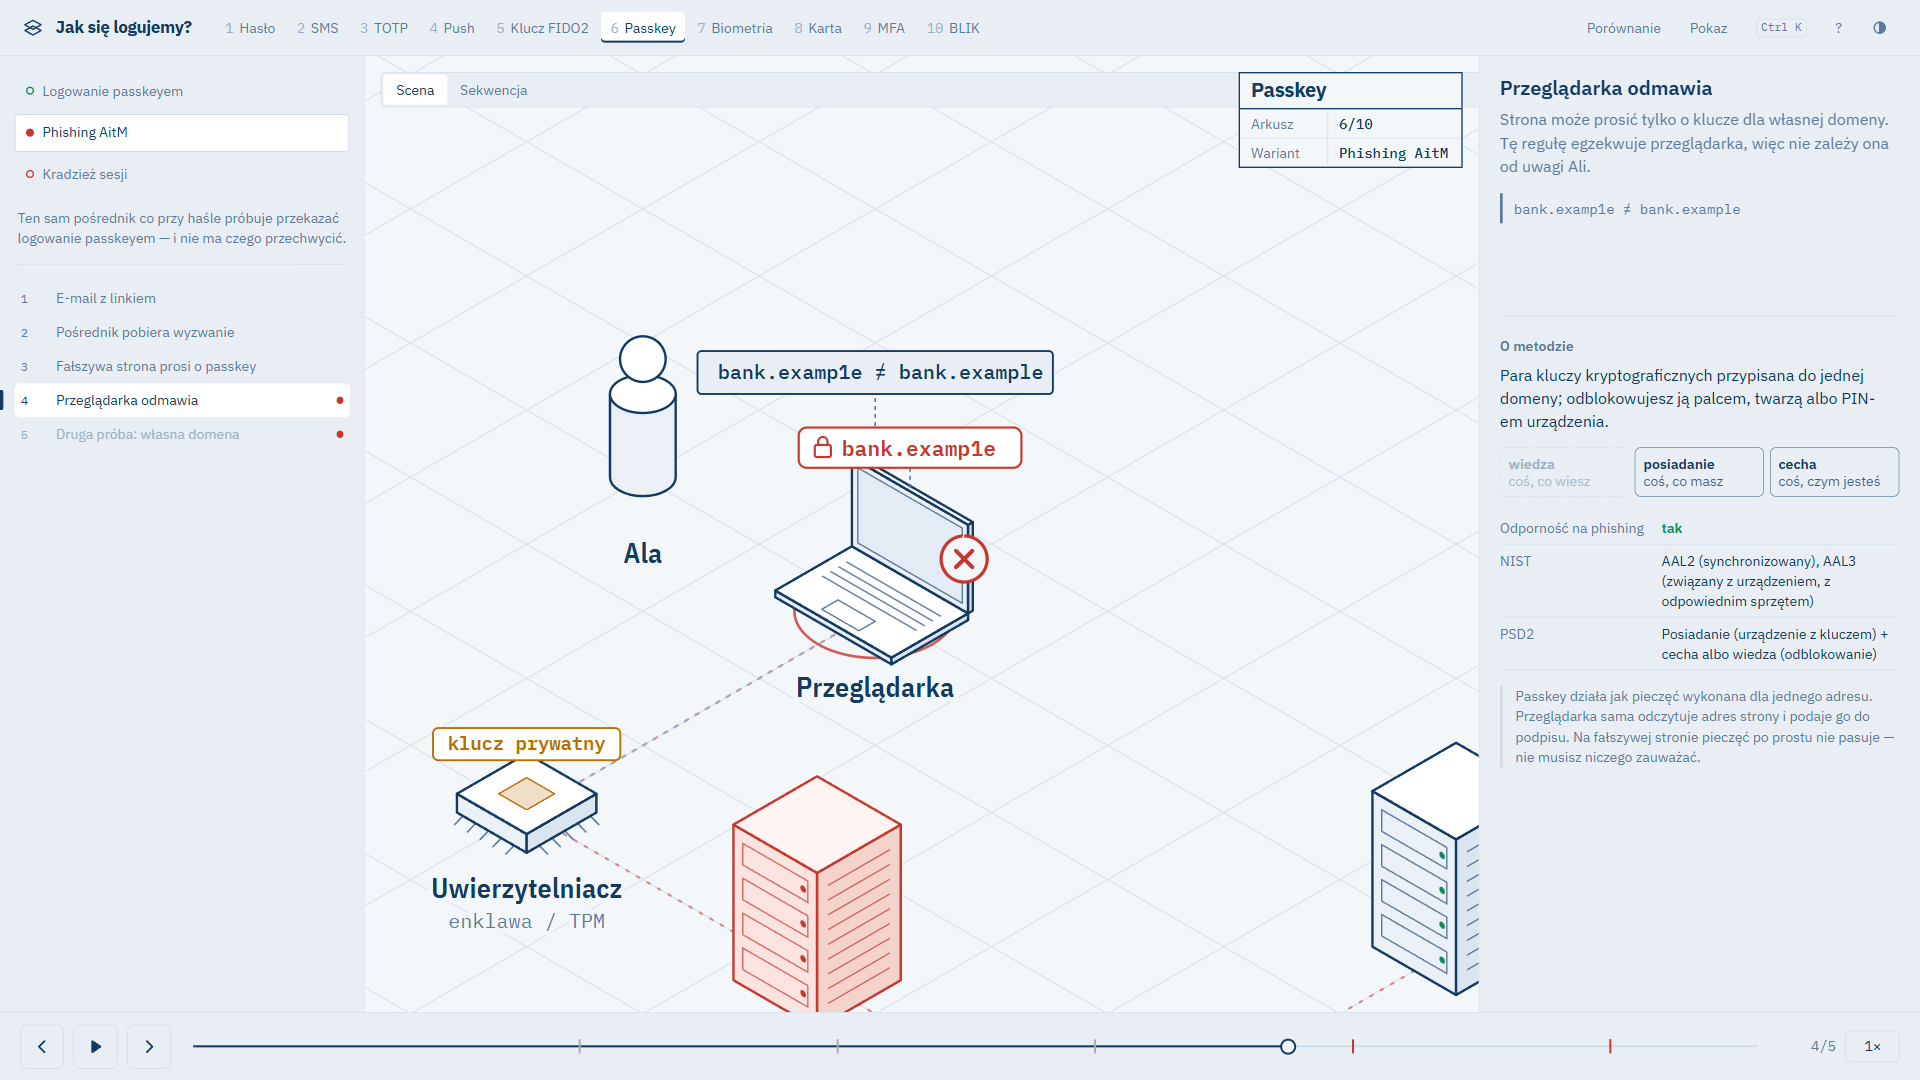
\includegraphics[width=\linewidth]{figures/explorer-passkey.png}
  \caption{Arkusz „Passkey”, wariant ataku phishingowego: przeglądarka odmawia podpisu, bo adres strony nie pasuje do domeny klucza.}
  \label{fig:explorer}
\end{figure}

\begin{figure}[ht]
  \centering
  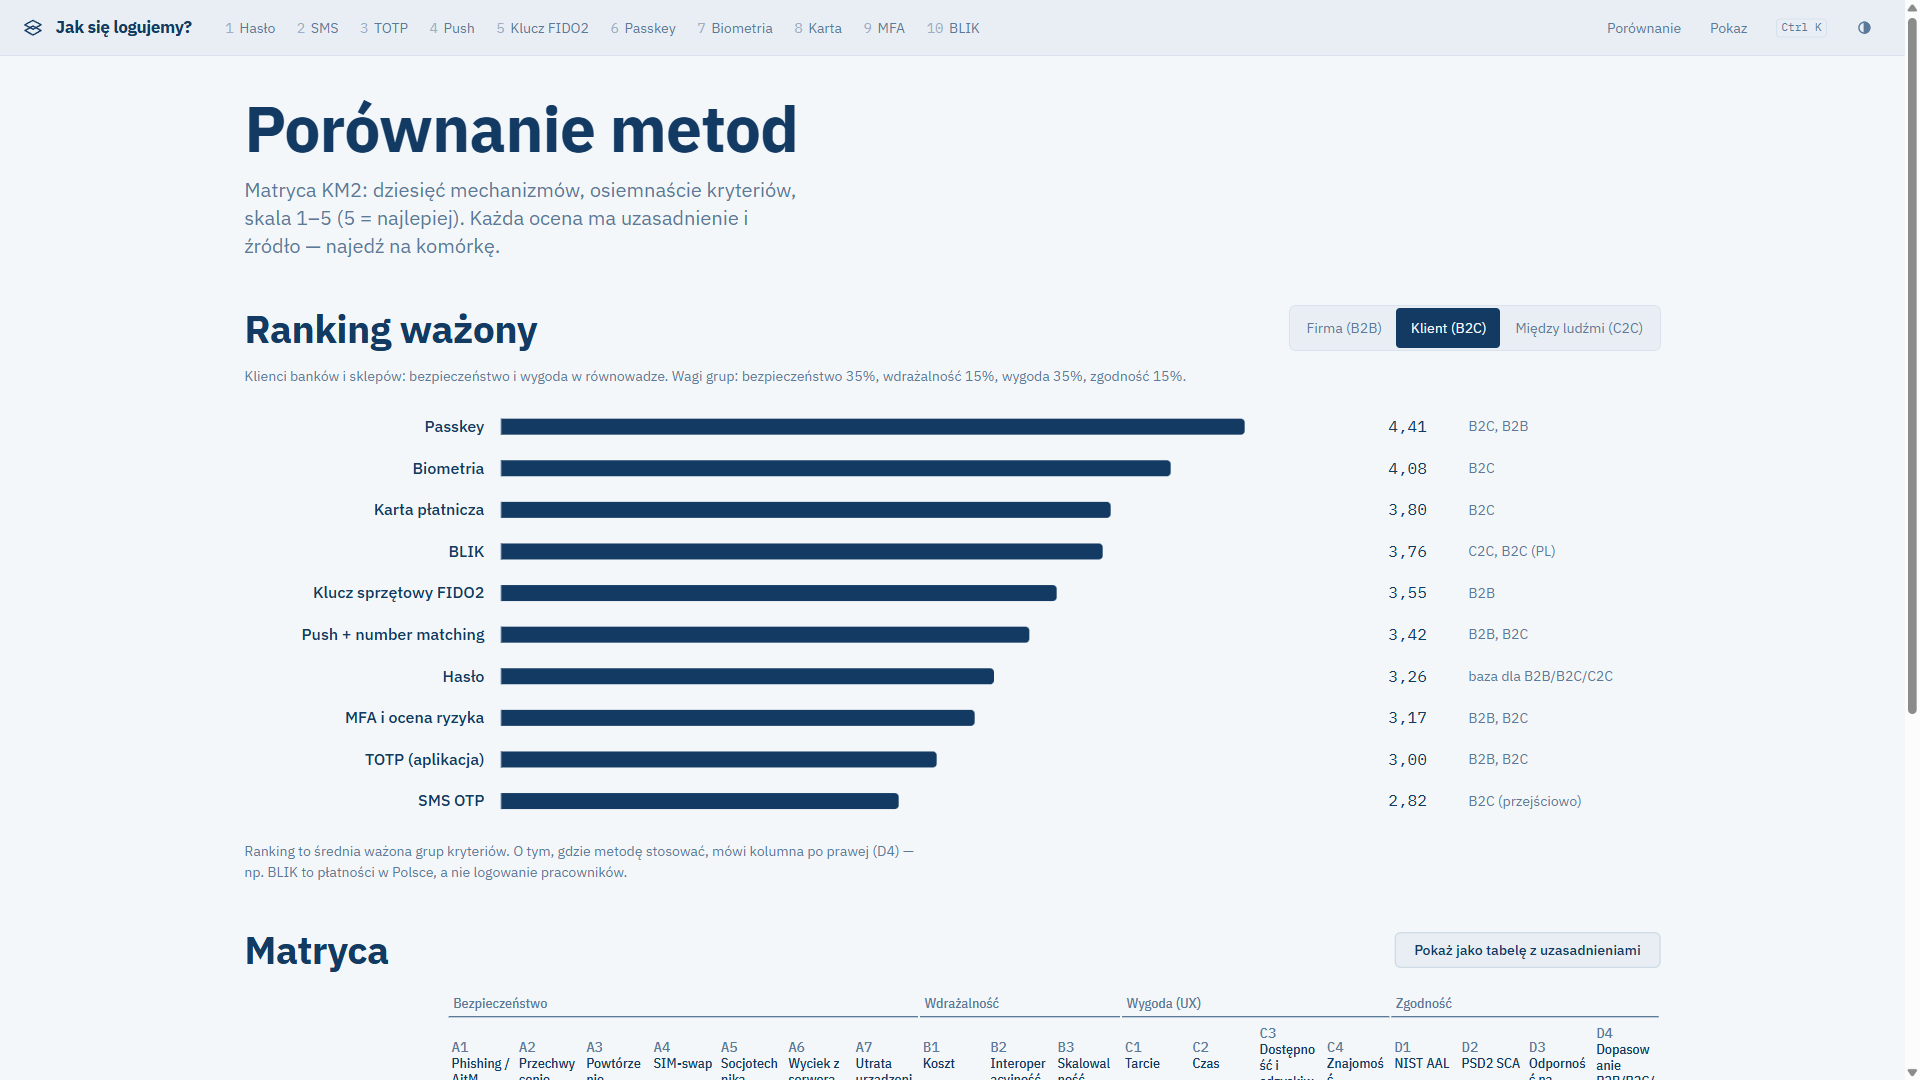
\includegraphics[width=\linewidth]{figures/porownanie.png}
  \caption{Widok porównania: ranking ważony i mapa ciepła matrycy.}
  \label{fig:porownanie}
\end{figure}

\begin{figure}[ht]
  \centering
  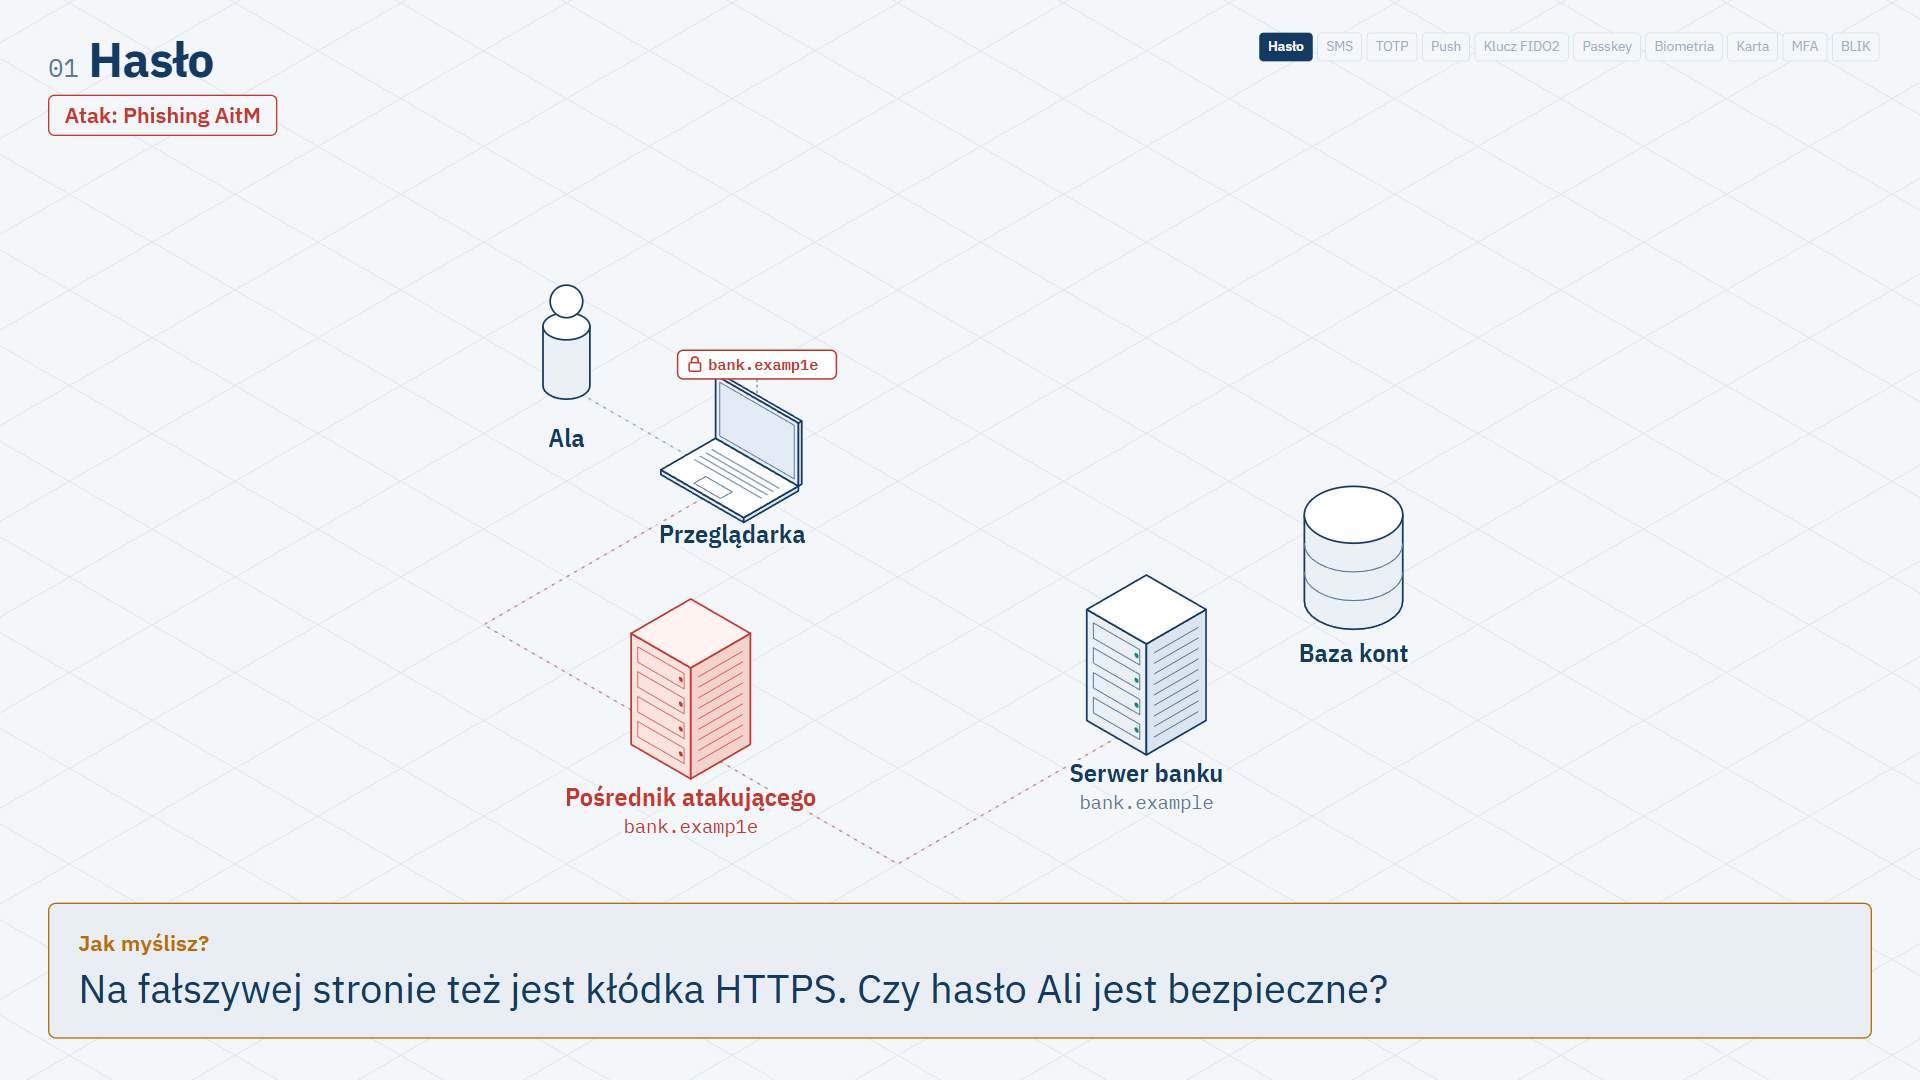
\includegraphics[width=0.49\linewidth]{figures/pokaz-pytanie.png}\hfill
  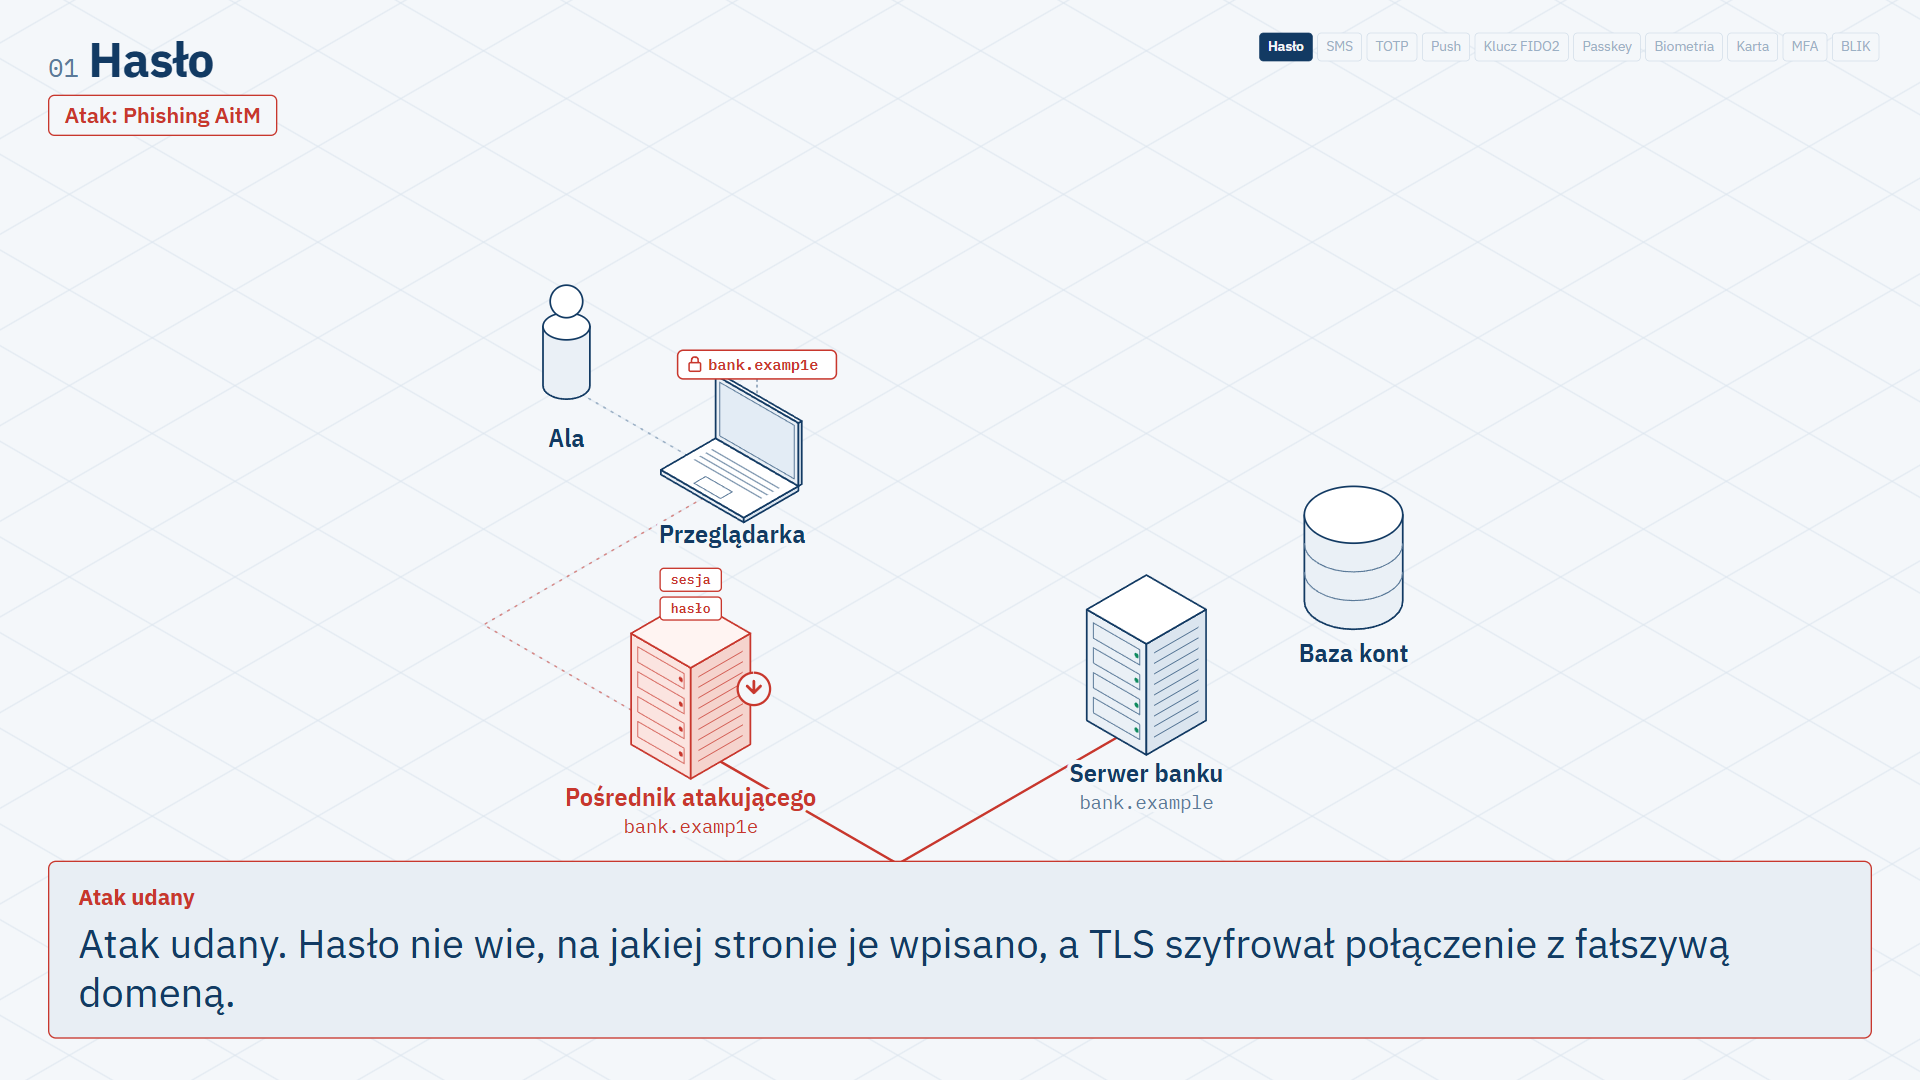
\includegraphics[width=0.49\linewidth]{figures/pokaz-werdykt.png}
  \caption{Pokaz: pytanie przed atakiem i werdykt po nim (arkusz „Hasło”, phishing AitM).}
  \label{fig:pokaz}
\end{figure}

\subsection{Założenia dydaktyczne}
Projekt opiera się na zasadach uczenia się z multimediów: segmentacji (krótkie kroki sterowane przez użytkownika), sygnalizacji (kolor i ruch tylko na tym, co zmienia stan), ciągłości przestrzennej (etykieta wiadomości jedzie razem z pakietem) i spójności (brak dekoracyjnej „hakerskiej” grafiki). Pytanie przed atakiem każe odbiorcy przewidzieć wynik, zanim go zobaczy, a odpowiedź wraca w werdykcie. Kolor niesie stałe znaczenie: zielony --- weryfikacja udana, bursztynowy --- sekret w ruchu, czerwony --- atakujący.

\subsection{Architektura}
Każda scena jest czystą funkcją czasu: dla danego mechanizmu, wariantu i chwili $t$ zwraca rysunek SVG. Dzięki temu ten sam kod napędza tryb interaktywny (czas z zegara przeglądarki, przewijanie, skoki między krokami), pokaz i wideo (czas z numeru klatki w Remotion). Rysunki izometryczne są składane z brył opisanych współrzędnymi siatki, więc pozostają ostre na ekranach 4K. Kod TOTP na arkuszu 3 jest obliczany naprawdę (HMAC-SHA-1 z sekretem z wektorów testowych RFC~6238).

Projekt jest inspirowany Protocol Explorer Diluma Sanjayi~\cite{W1} (informacja także w aplikacji). Kod, rysunki i treść powstały od podstaw.

% ─────────────────────────────────────────────────────────────
\section{Wnioski}

\begin{enumerate}
  \item Odporność na phishing pośredniczący zapewnia protokół. Spośród badanych mechanizmów mają ją tylko te oparte na WebAuthn (passkey, klucz FIDO2): wiążą podpis z domeną, a adres sprawdza przeglądarka, więc wynik nie zależy od uwagi użytkownika.
  \item Mechanizmy oparte na kodach (SMS, TOTP) i prostych zatwierdzeniach (push bez dopasowania liczby) chronią przed odgadnięciem i wyciekiem hasła, ale nie przed pośrednikiem i socjotechniką. SMS dodatkowo zależy od bezpieczeństwa operatora.
  \item Najlepszy kompromis bezpieczeństwa i wygody daje passkey. Klucz FIDO2 jest najbezpieczniejszy, ale opłaca się głównie w B2B i dla kont uprzywilejowanych.
  \item Bezpieczeństwo wdrożenia wyznacza najsłabsza dostępna ścieżka: metoda zapasowa, odzyskiwanie konta, sesja po zalogowaniu.
  \item W płatnościach technika (EMV, BLIK z dynamicznym powiązaniem) jest dojrzała; dominujące ataki --- przekaźnik NFC, „pożycz na BLIKa” --- wykorzystują człowieka. Edukacja jest tu równie ważna jak protokół.
\end{enumerate}

\printbibliography[heading=bibintoc,title={Bibliografia}]

\appendix
\section{Uzasadnienia ocen}\label{app:uzasadnienia}
% Plik generowany: npm --prefix 04_app run gen:report — nie edytować ręcznie.
\subsection*{1. Hasło}
\begingroup\small
\begin{longtable}{@{}p{0.2\linewidth}c p{0.56\linewidth}l@{}}
\toprule
Kryterium & Ocena & Uzasadnienie & Źródła \\
\midrule
\endhead
A1 Phishing / AitM & 1 & Hasło działa na każdej stronie, na której zostanie wpisane; pośrednik przekazuje je bez przeszkód. & \cite{A1,P6} \\
A2 Przechwycenie kanału & 3 & TLS chroni hasło w drodze, ale po stronie serwera jest ono przez chwilę jawne. & \cite{N1,N4} \\
A3 Powtórzenie & 1 & Przechwycone hasło działa wielokrotnie aż do zmiany. & \cite{P6,X1} \\
A4 SIM-swap & 4 & Nie zależy od numeru telefonu, o ile reset hasła nie idzie przez SMS. & \cite{N1,P11} \\
A5 Socjotechnika & 1 & Hasło można po prostu wyłudzić lub podyktować. & \cite{N5,P6} \\
A6 Wyciek z serwera & 2 & Sól i Argon2id spowalniają łamanie, ale słabe i powtarzane hasła padają po wycieku. & \cite{X3,X4} \\
A7 Utrata urządzenia & 4 & Nie jest związane z urządzeniem; ryzyko tylko przy hasłach zapisanych bez blokady. & \cite{N1} \\
B1 Koszt & 5 & Brak sprzętu i opłat; standard każdego frameworka. & \cite{X1,P7} \\
B2 Interoperacyjność & 5 & Działa wszędzie, na każdym urządzeniu. & \cite{X1} \\
B3 Skalowalność & 5 & Skaluje się bez logistyki; koszty to głównie obsługa resetów. & \cite{X1} \\
C1 Tarcie & 4 & Jeden krok, ale wymaga pamiętania lub menedżera haseł. & \cite{P8,X1} \\
C2 Czas & 4 & Kilka sekund z menedżerem haseł, dłużej bez niego. & \cite{P1} \\
C3 Dostępność i odzyskiwanie & 4 & Łatwe odzyskanie przez e-mail, choć sam reset bywa słabym punktem. & \cite{P11} \\
C4 Znajomość & 5 & Najlepiej znana metoda. & \cite{P8,X1} \\
D1 NIST AAL & AAL1 (2) & Samo hasło to AAL1. & \cite{N1} \\
D2 PSD2 SCA & nie (1) & Jeden element (wiedza) — nie spełnia SCA. & \cite{N3} \\
D3 Odporność na phishing & nie (1) & Nie jest odporne na phishing. & \cite{N1,P6} \\
D4 Dopasowanie B2B/B2C/C2C & baza dla B2B/B2C/C2C (2) & Wszędzie jako baza, ale nie jako jedyny składnik przy transakcjach. & \cite{N3,N4} \\
\bottomrule
\end{longtable}
\endgroup

\subsection*{2. SMS OTP}
\begingroup\small
\begin{longtable}{@{}p{0.2\linewidth}c p{0.56\linewidth}l@{}}
\toprule
Kryterium & Ocena & Uzasadnienie & Źródła \\
\midrule
\endhead
A1 Phishing / AitM & 1 & Pośrednik przekazuje kod w czasie jego ważności. & \cite{A1,A3} \\
A2 Przechwycenie kanału & 2 & SMS nie jest szyfrowany end-to-end; możliwe przechwycenie w sieci (SS7) lub przez złośliwe aplikacje. & \cite{A3,N1} \\
A3 Powtórzenie & 4 & Kod jednorazowy i krótko ważny. & \cite{N1,P7} \\
A4 SIM-swap & 1 & Przejęcie numeru (SIM-swap) daje dostęp do kodów. & \cite{X2,A3,X8} \\
A5 Socjotechnika & 2 & Kod łatwo podyktować „pracownikowi banku”. & \cite{A3,P9} \\
A6 Wyciek z serwera & 4 & Serwer przechowuje tylko numer telefonu; kody są ulotne. & \cite{N1} \\
A7 Utrata urządzenia & 2 & Kod często widać na zablokowanym ekranie. & \cite{A3} \\
B1 Koszt & 3 & Opłaty za każdą wiadomość, rosnące przy ruchu międzynarodowym. & \cite{P7,A3} \\
B2 Interoperacyjność & 5 & Działa na każdym telefonie komórkowym. & \cite{P7,P8} \\
B3 Skalowalność & 3 & Zależność od operatorów i opóźnień doręczenia. & \cite{P7} \\
C1 Tarcie & 2 & Oczekiwanie na SMS i przepisywanie kodu. & \cite{P8,P12} \\
C2 Czas & 2 & Kilkanaście sekund do minut, zależnie od doręczenia. & \cite{P8} \\
C3 Dostępność i odzyskiwanie & 4 & Nie wymaga smartfona; łatwa zmiana numeru. & \cite{P7,P9} \\
C4 Znajomość & 5 & Bardzo dobrze znana metoda. & \cite{P8,P9} \\
D1 NIST AAL & AAL2 (restricted) (2) & AAL2, ale NIST oznacza ją jako „restricted”. & \cite{N1} \\
D2 PSD2 SCA & tak (z hasłem) (4) & Z hasłem spełnia SCA; kwota może być w treści SMS. & \cite{N3} \\
D3 Odporność na phishing & nie (1) & Nie jest odporny na phishing. & \cite{N1,A1} \\
D4 Dopasowanie B2B/B2C/C2C & B2C (przejściowo) (2) & B2C przejściowo; odchodzi się od niego w bankowości. & \cite{N1,R2} \\
\bottomrule
\end{longtable}
\endgroup

\subsection*{3. TOTP (aplikacja)}
\begingroup\small
\begin{longtable}{@{}p{0.2\linewidth}c p{0.56\linewidth}l@{}}
\toprule
Kryterium & Ocena & Uzasadnienie & Źródła \\
\midrule
\endhead
A1 Phishing / AitM & 1 & Kod jest ważny ok. 30–90 s; pośrednik zdąży go użyć. & \cite{A1,S3} \\
A2 Przechwycenie kanału & 4 & Sekret nie krąży po sieci po rejestracji; kod idzie przez TLS. & \cite{S3,N1} \\
A3 Powtórzenie & 4 & Kod ważny tylko w oknie czasowym; poprawna implementacja odrzuca ponowne użycie. & \cite{S3,S4} \\
A4 SIM-swap & 5 & Nie zależy od numeru telefonu. & \cite{S3,P7} \\
A5 Socjotechnika & 2 & Kod można podyktować oszustowi. & \cite{P9,A1} \\
A6 Wyciek z serwera & 2 & Serwer przechowuje wspólny sekret; jego wyciek pozwala liczyć kody. & \cite{S3,N1} \\
A7 Utrata urządzenia & 3 & Aplikacja często nie ma osobnej blokady. & \cite{N4} \\
B1 Koszt & 5 & Darmowe aplikacje, otwarty standard. & \cite{S3,P7} \\
B2 Interoperacyjność & 4 & Standard RFC obsługiwany przez wiele aplikacji. & \cite{S3} \\
B3 Skalowalność & 5 & Brak opłat za wiadomości i zależności od operatora. & \cite{S3} \\
C1 Tarcie & 2 & Otwarcie aplikacji i przepisanie kodu. & \cite{P8,P4} \\
C2 Czas & 3 & Kilka do kilkunastu sekund. & \cite{P8} \\
C3 Dostępność i odzyskiwanie & 2 & Utrata telefonu bez kopii sekretu blokuje dostęp. & \cite{P11} \\
C4 Znajomość & 3 & Mniej znana niż SMS. & \cite{P8,P9} \\
D1 NIST AAL & AAL2 (3) & AAL2. & \cite{N1} \\
D2 PSD2 SCA & częściowo (3) & Z hasłem spełnia SCA przy logowaniu; brak powiązania z kwotą transakcji. & \cite{N3} \\
D3 Odporność na phishing & nie (1) & Nie jest odporny na phishing. & \cite{N1,A1} \\
D4 Dopasowanie B2B/B2C/C2C & B2B, B2C (3) & B2B i B2C jako drugi składnik. & \cite{N4,P7} \\
\bottomrule
\end{longtable}
\endgroup

\subsection*{4. Push + number matching}
\begingroup\small
\begin{longtable}{@{}p{0.2\linewidth}c p{0.56\linewidth}l@{}}
\toprule
Kryterium & Ocena & Uzasadnienie & Źródła \\
\midrule
\endhead
A1 Phishing / AitM & 2 & Dopasowanie liczby nie blokuje pośrednika, który pokazuje ofierze prawdziwą liczbę. & \cite{A1,X5} \\
A2 Przechwycenie kanału & 4 & Kanał TLS, odpowiedź podpisana kluczem urządzenia. & \cite{X9,P10} \\
A3 Powtórzenie & 5 & Każde potwierdzenie dotyczy jednej próby logowania. & \cite{X9} \\
A4 SIM-swap & 4 & Nie zależy od SMS, chyba że aktywacja na nowym telefonie idzie przez SMS. & \cite{P11,X5} \\
A5 Socjotechnika & 3 & Dopasowanie liczby zatrzymuje push bombing; zostaje socjotechnika przez telefon. & \cite{A2,X5,X9} \\
A6 Wyciek z serwera & 5 & Serwer zna tylko klucz publiczny urządzenia. & \cite{X9} \\
A7 Utrata urządzenia & 4 & Aplikacja chroniona PIN-em lub biometrią. & \cite{P10} \\
B1 Koszt & 3 & Wymaga własnej aplikacji albo dostawcy tożsamości. & \cite{P7,P10} \\
B2 Interoperacyjność & 2 & Zależy od aplikacji konkretnego dostawcy. & \cite{P10} \\
B3 Skalowalność & 4 & Dobrze skaluje się w firmach i bankach z aplikacją. & \cite{P10} \\
C1 Tarcie & 3 & Dopasowanie liczby dodaje krok, ale bez przepisywania długiego kodu. & \cite{X5,X9} \\
C2 Czas & 3 & Kilka sekund, zależnie od dostarczenia powiadomienia. & \cite{X9} \\
C3 Dostępność i odzyskiwanie & 3 & Wymaga smartfona; zmiana telefonu wymaga ponownej aktywacji. & \cite{P11} \\
C4 Znajomość & 4 & Powszechne w bankowości mobilnej. & \cite{P9} \\
D1 NIST AAL & AAL2 (3) & AAL2. & \cite{N1} \\
D2 PSD2 SCA & tak (5) & Spełnia SCA, w aplikacji można pokazać kwotę i odbiorcę. & \cite{N3} \\
D3 Odporność na phishing & nie (1) & Nie jest odporny na phishing AitM. & \cite{N1,X5} \\
D4 Dopasowanie B2B/B2C/C2C & B2B, B2C (4) & B2B (pracownicy) i B2C (banki). & \cite{P10,X9} \\
\bottomrule
\end{longtable}
\endgroup

\subsection*{5. Klucz sprzętowy FIDO2}
\begingroup\small
\begin{longtable}{@{}p{0.2\linewidth}c p{0.56\linewidth}l@{}}
\toprule
Kryterium & Ocena & Uzasadnienie & Źródła \\
\midrule
\endhead
A1 Phishing / AitM & 5 & Podpis związany z domeną; przeglądarka egzekwuje origin. & \cite{S1,A1,P6} \\
A2 Przechwycenie kanału & 5 & Kanał niczego nie zdradza: podpis jest jednorazowy i związany z domeną. & \cite{S1,S2} \\
A3 Powtórzenie & 5 & Wyzwanie serwera i licznik podpisów uniemożliwiają powtórzenie. & \cite{S1,S2} \\
A4 SIM-swap & 5 & Nie zależy od telefonu. & \cite{P6} \\
A5 Socjotechnika & 4 & Nie ma kodu do podyktowania; zostaje wyłudzenie rejestracji lub odzyskiwania. & \cite{P6,P11} \\
A6 Wyciek z serwera & 5 & Serwer przechowuje tylko klucze publiczne. & \cite{P6,S1} \\
A7 Utrata urządzenia & 4 & Klucz bez PIN-u jest bezużyteczny; blokada po 8 próbach. & \cite{S2} \\
B1 Koszt & 1 & Zakup sprzętu dla każdego użytkownika, zwykle dwóch sztuk. & \cite{P3,P7} \\
B2 Interoperacyjność & 4 & WebAuthn w głównych przeglądarkach; wymaga USB/NFC. & \cite{S1,P2} \\
B3 Skalowalność & 2 & Logistyka dystrybucji i wymiany kluczy. & \cite{P3} \\
C1 Tarcie & 3 & Podłączenie, PIN i dotyk. & \cite{P1,P2} \\
C2 Czas & 3 & Kilka sekund; szybsze bez PIN-u. & \cite{P1} \\
C3 Dostępność i odzyskiwanie & 2 & Zgubiony klucz wymaga zapasowego klucza lub procedury odzyskiwania. & \cite{P3,P11} \\
C4 Znajomość & 2 & Użytkownicy słabo rozumieją przewagę klucza nad innymi metodami. & \cite{P3,P1} \\
D1 NIST AAL & AAL3 (5) & AAL3 przy certyfikowanym sprzęcie. & \cite{N1} \\
D2 PSD2 SCA & tak (bez powiązania z kwotą) (4) & Posiadanie + wiedza; powiązanie z transakcją wymaga dodatkowego rozszerzenia. & \cite{N3,S1} \\
D3 Odporność na phishing & tak (5) & Odporny na phishing. & \cite{N1,P6} \\
D4 Dopasowanie B2B/B2C/C2C & B2B (4) & Przede wszystkim B2B i konta uprzywilejowane. & \cite{P3,R2} \\
\bottomrule
\end{longtable}
\endgroup

\subsection*{6. Passkey}
\begingroup\small
\begin{longtable}{@{}p{0.2\linewidth}c p{0.56\linewidth}l@{}}
\toprule
Kryterium & Ocena & Uzasadnienie & Źródła \\
\midrule
\endhead
A1 Phishing / AitM & 5 & Podpis związany z domeną; fałszywa strona nie dostanie ważnego podpisu. & \cite{S1,P6,A1} \\
A2 Przechwycenie kanału & 5 & Podpis jednorazowy; synchronizacja kluczy szyfrowana end-to-end. & \cite{S1,P5} \\
A3 Powtórzenie & 5 & Wyzwanie serwera wyklucza powtórzenie. & \cite{S1} \\
A4 SIM-swap & 4 & Odzyskanie konta chmurowego bywa oparte na SMS. & \cite{P5,P11} \\
A5 Socjotechnika & 4 & Brak kodu do podyktowania; ryzyko przy odzyskiwaniu konta. & \cite{P4,P11} \\
A6 Wyciek z serwera & 5 & Serwer przechowuje tylko klucze publiczne. & \cite{S1,P6} \\
A7 Utrata urządzenia & 4 & Użycie wymaga odblokowania urządzenia. & \cite{S1,P5} \\
B1 Koszt & 4 & Wbudowane w systemy; koszt to praca wdrożeniowa. & \cite{P4,R2} \\
B2 Interoperacyjność & 4 & Wspierane przez główne platformy, choć ekosystemy synchronizacji są rozłączne. & \cite{P4,P5,W4} \\
B3 Skalowalność & 5 & Brak sprzętu do dystrybucji. & \cite{R2,P4} \\
C1 Tarcie & 5 & Jeden gest: palec, twarz albo PIN urządzenia. & \cite{P4,P1} \\
C2 Czas & 5 & Najkrótsze logowanie spośród badanych metod. & \cite{P4,R2} \\
C3 Dostępność i odzyskiwanie & 4 & Synchronizacja ułatwia odzyskanie; wersja związana z urządzeniem trudniejsza. & \cite{P5} \\
C4 Znajomość & 3 & Znajomość rośnie (57\% w 2024 r.), ale nadal ograniczona. & \cite{R1,R2} \\
D1 NIST AAL & AAL2/AAL3 (4) & AAL2 (synchronizowany), AAL3 (związany z urządzeniem). & \cite{N1} \\
D2 PSD2 SCA & tak (bez powiązania z kwotą) (4) & Posiadanie + cecha lub wiedza; powiązanie z kwotą wymaga dodatkowego rozszerzenia. & \cite{N3,S1} \\
D3 Odporność na phishing & tak (5) & Odporny na phishing. & \cite{N1,P6} \\
D4 Dopasowanie B2B/B2C/C2C & B2C, B2B (5) & B2C (synchronizowane) i B2B (związane z urządzeniem). & \cite{R2,P5} \\
\bottomrule
\end{longtable}
\endgroup

\subsection*{7. Biometria}
\begingroup\small
\begin{longtable}{@{}p{0.2\linewidth}c p{0.56\linewidth}l@{}}
\toprule
Kryterium & Ocena & Uzasadnienie & Źródła \\
\midrule
\endhead
A1 Phishing / AitM & 4 & Brak sekretu do wpisania; odporność zależy od odblokowywanego uwierzytelniacza. & \cite{S1,N1} \\
A2 Przechwycenie kanału & 5 & Wzorzec nie opuszcza urządzenia. & \cite{N1,P13} \\
A3 Powtórzenie & 3 & Słabe czujniki można oszukać nagraną próbką; pomaga challenge-response. & \cite{P16,P13} \\
A4 SIM-swap & 5 & Niezależna od telefonu jako numeru. & \cite{N1} \\
A5 Socjotechnika & 4 & Trudno ją „podyktować”; możliwe wymuszenie fizyczne. & \cite{P13} \\
A6 Wyciek z serwera & 5 & Wzorzec przechowywany lokalnie, nie na serwerze. & \cite{N1,S1} \\
A7 Utrata urządzenia & 4 & Test żywotności i limit prób, potem PIN. & \cite{P14,N6} \\
B1 Koszt & 4 & Czytniki wbudowane w telefony i laptopy. & \cite{P15} \\
B2 Interoperacyjność & 3 & Zależy od urządzenia i czujnika. & \cite{P13,P2} \\
B3 Skalowalność & 4 & Skaluje się z urządzeniami użytkowników. & \cite{P15} \\
C1 Tarcie & 5 & Jeden gest. & \cite{P15,P2} \\
C2 Czas & 5 & Ułamek sekundy. & \cite{P15} \\
C3 Dostępność i odzyskiwanie & 3 & Nie dla każdego (np. starte linie papilarne); potrzebny PIN zapasowy. & \cite{P15,P13} \\
C4 Znajomość & 5 & Powszechna w telefonach. & \cite{P15} \\
D1 NIST AAL & n/d samodzielnie (2) & Według NIST tylko w połączeniu z fizycznym uwierzytelniaczem. & \cite{N1} \\
D2 PSD2 SCA & częściowo (3) & Element „cecha”; potrzebny drugi element. & \cite{N3} \\
D3 Odporność na phishing & częściowo (3) & Zależy od uwierzytelniacza, który odblokowuje. & \cite{N1} \\
D4 Dopasowanie B2B/B2C/C2C & B2C (4) & B2C jako odblokowanie passkeya i aplikacji. & \cite{P15,R2} \\
\bottomrule
\end{longtable}
\endgroup

\subsection*{8. Karta płatnicza}
\begingroup\small
\begin{longtable}{@{}p{0.2\linewidth}c p{0.56\linewidth}l@{}}
\toprule
Kryterium & Ocena & Uzasadnienie & Źródła \\
\midrule
\endhead
A1 Phishing / AitM & 3 & Chipu nie da się sphishować przy kasie, ale dane karty wyłudza się do płatności online. & \cite{A6,S5} \\
A2 Przechwycenie kanału & 3 & Kryptogram EMV jest bezwartościowy dla podsłuchującego; pasek — nie. & \cite{A9,A8} \\
A3 Powtórzenie & 3 & Chip: licznik i liczba losowa; pasek: dane statyczne. & \cite{A6,A8} \\
A4 SIM-swap & 5 & Niezależna od telefonu. & \cite{S5} \\
A5 Socjotechnika & 3 & Ofiarę namawia się do przyłożenia karty do telefonu i podania PIN-u. & \cite{X6} \\
A6 Wyciek z serwera & 3 & Klucze w HSM banku; wycieki u sprzedawców ujawniają numery do płatności online. & \cite{A6} \\
A7 Utrata urządzenia & 2 & Płatności zbliżeniowe bez PIN-u do limitu; obejścia PIN w niektórych konfiguracjach. & \cite{A4,A6} \\
B1 Koszt & 2 & Karty, terminale, sieć płatnicza, HSM. & \cite{S5,A6} \\
B2 Interoperacyjność & 5 & Globalna akceptacja EMV. & \cite{S5} \\
B3 Skalowalność & 4 & Dojrzała infrastruktura, ale wymiana kart kosztuje. & \cite{S5} \\
C1 Tarcie & 5 & Przyłożenie karty. & \cite{S5} \\
C2 Czas & 5 & Około sekundy. & \cite{S5} \\
C3 Dostępność i odzyskiwanie & 4 & Bank wydaje nową kartę. & \cite{S5} \\
C4 Znajomość & 5 & Powszechnie znana. & \cite{S5} \\
D1 NIST AAL & n/d (3) & Nie dotyczy (płatności, nie logowanie). & \cite{N1} \\
D2 PSD2 SCA & częściowo (3) & Z PIN-em spełnia SCA; drobne płatności zbliżeniowe są zwolnione. & \cite{N3} \\
D3 Odporność na phishing & częściowo (3) & Chip odporny na powtórzenie, pasek i przekaźnik nie. & \cite{A5,A6} \\
D4 Dopasowanie B2B/B2C/C2C & B2C (4) & B2C w handlu. & \cite{S5,N7} \\
\bottomrule
\end{longtable}
\endgroup

\subsection*{9. MFA i ocena ryzyka}
\begingroup\small
\begin{longtable}{@{}p{0.2\linewidth}c p{0.56\linewidth}l@{}}
\toprule
Kryterium & Ocena & Uzasadnienie & Źródła \\
\midrule
\endhead
A1 Phishing / AitM & 3 & Zależy od składników: z passkeyem odporne, z hasłem i kodem nie. & \cite{A1,N4} \\
A2 Przechwycenie kanału & 4 & Kilka niezależnych kanałów utrudnia przechwycenie. & \cite{N4,P10} \\
A3 Powtórzenie & 4 & Składniki dynamiczne wykluczają powtórzenie. & \cite{N4} \\
A4 SIM-swap & 3 & Słabe, jeśli SMS jest jednym ze składników lub ścieżką zapasową. & \cite{P11,X2} \\
A5 Socjotechnika & 3 & Wymaga oszukania na więcej niż jednym etapie; zmęczenie użytkownika zostaje. & \cite{A2,P9} \\
A6 Wyciek z serwera & 4 & Wyciek jednego składnika nie wystarcza. & \cite{N4} \\
A7 Utrata urządzenia & 4 & Utrata jednego urządzenia nie daje dostępu. & \cite{N4} \\
B1 Koszt & 3 & Koszt sumy składników i systemu oceny ryzyka. & \cite{P10,P7} \\
B2 Interoperacyjność & 3 & Zależy od wybranych składników. & \cite{P12} \\
B3 Skalowalność & 4 & Dobrze skaluje się z oceną ryzyka (więcej kroków tylko przy ryzyku). & \cite{P10} \\
C1 Tarcie & 2 & Kilka kroków przy logowaniu. & \cite{P9,P8} \\
C2 Czas & 2 & Najdłużej spośród badanych. & \cite{P8} \\
C3 Dostępność i odzyskiwanie & 2 & Odzyskiwanie bywa skomplikowane i osłabia całość. & \cite{P11} \\
C4 Znajomość & 3 & Znane, ale obowiązkowe MFA bez edukacji bywa nieskuteczne. & \cite{P9} \\
D1 NIST AAL & AAL2–AAL3 (4) & AAL2–AAL3 zależnie od składników. & \cite{N1} \\
D2 PSD2 SCA & tak (5) & To definicja SCA. & \cite{N3} \\
D3 Odporność na phishing & częściowo (3) & Tylko gdy składnik jest odporny na phishing. & \cite{N1,A1} \\
D4 Dopasowanie B2B/B2C/C2C & B2B, B2C (5) & B2B i B2C przy wysokiej stawce. & \cite{N4,N7} \\
\bottomrule
\end{longtable}
\endgroup

\subsection*{10. BLIK}
\begingroup\small
\begin{longtable}{@{}p{0.2\linewidth}c p{0.56\linewidth}l@{}}
\toprule
Kryterium & Ocena & Uzasadnienie & Źródła \\
\midrule
\endhead
A1 Phishing / AitM & 3 & Kod wyłudzany na fałszywych stronach płatności, ale potwierdzenie pokazuje kwotę i odbiorcę. & \cite{X7,N3} \\
A2 Przechwycenie kanału & 4 & Kod bez potwierdzenia w aplikacji jest bezużyteczny. & \cite{X7} \\
A3 Powtórzenie & 5 & Kod jednorazowy, 2 minuty, potwierdzenie każdej transakcji. & \cite{X7} \\
A4 SIM-swap & 4 & Aktywacja aplikacji na nowym telefonie wymaga logowania do banku. & \cite{X7,X2} \\
A5 Socjotechnika & 2 & Główny wektor oszustw: „pożycz na BLIKa”, fałszywe „odbieranie płatności”. & \cite{X7,P9} \\
A6 Wyciek z serwera & 5 & Kody ulotne; bank przechowuje klucz publiczny aplikacji. & \cite{X7} \\
A7 Utrata urządzenia & 4 & Aplikacja chroniona PIN-em lub biometrią. & \cite{X7} \\
B1 Koszt & 3 & Tanio dla sprzedawców; banki potrzebują integracji z systemem BLIK. & \cite{X7} \\
B2 Interoperacyjność & 2 & Głównie Polska. & \cite{X7} \\
B3 Skalowalność & 4 & Działa w skali krajowej. & \cite{X7} \\
C1 Tarcie & 4 & Kod i jedno potwierdzenie. & \cite{X7} \\
C2 Czas & 4 & Kilka sekund. & \cite{X7} \\
C3 Dostępność i odzyskiwanie & 3 & Wymaga smartfona i aplikacji polskiego banku. & \cite{X7} \\
C4 Znajomość & 5 & Powszechny w Polsce. & \cite{X7} \\
D1 NIST AAL & n/d (3) & Nie dotyczy (płatności). & \cite{N1} \\
D2 PSD2 SCA & tak (5) & Spełnia SCA z dynamicznym powiązaniem. & \cite{N3,X7} \\
D3 Odporność na phishing & częściowo (3) & Potwierdzenie z kwotą pomaga, ale zależy od uwagi użytkownika. & \cite{X7} \\
D4 Dopasowanie B2B/B2C/C2C & C2C, B2C (PL) (4) & C2C i B2C w Polsce. & \cite{X7} \\
\bottomrule
\end{longtable}
\endgroup


\end{document}
